% \PassOptionsToPackage{pdftex}{graphicx}
\PassOptionsToPackage{table,xcdraw}{xcolor}
\documentclass[journal,10pt,compsoc]{IEEEtran}

%! suppress = MissingImport
\usepackage[utf8]{inputenc}
\usepackage[T1]{fontenc}
\usepackage[htt]{hyphenat}  % for linebreaks in texttt
\usepackage{import}
\usepackage[pdftex]{graphicx}
\usepackage{indentfirst}
\graphicspath{{./images/}{./plots/}{./figures}}
\DeclareGraphicsExtensions{.pdf,.jpeg,.png}
\usepackage[tbtags]{amsmath}
\usepackage{relsize}
\usepackage{mathtools}
\usepackage{amssymb}
\usepackage[d]{esvect}
\usepackage{url}
\usepackage{orcidlink}
\usepackage{caption}
\usepackage[subrefformat=parens]{subcaption}
\usepackage{booktabs}
\usepackage{multirow}
\usepackage{makecell}
\usepackage{tabularx}
\usepackage[all]{hypcap}
\usepackage[newfloat]{minted} % must be loaded after amsmath
\usepackage[capitalize,nameinlink,noabbrev]{cleveref}
\usepackage[table,xcdraw]{xcolor}
\usepackage[detect-weight=true,detect-family=true,binary-units=true,list-units=single,range-units=single]{siunitx}
\sisetup{list-final-separator = {, and }}
\usepackage[nogroupskip,nonumberlist,shortcuts,acronym]{glossaries-extra}
\usepackage{glossaries-prefix}
\newcommand*\dif{\,\mathrm{d}}
\newcommand*\df{\mathrm{d}}
\newcommand*\ts{T_{\text{s}}}
\usepackage[
    style=numeric-comp,
    sorting=none,
    sortcites,
    hyperref,
    mincitenames=1,
    maxcitenames=2,
    maxbibnames=2,
    minbibnames=1,
    citestyle=numeric-comp, % for [1, 2] instead of [1], [2]
    backend=biber
]{biblatex}
\usepackage[inline]{enumitem}
\usepackage{todonotes}

\SetupFloatingEnvironment{listing}{name=List.,within=none}

% enumitem
\newlist{inlineenum}{enumerate*}{1}
\setlist*[inlineenum]{
    label=(\arabic*),
    itemjoin={{; }},
    itemjoin*={{; and }},
}
\setlist[description]{font=\normalfont\underline}


% glossary settings
% \setglossarystyle{mcolindexgroup}
\setabbreviationstyle[acronym]{long-short-user}
% \glstoctrue%
\makeglossaries%
\newcommand*\nestedgls[1]{%
  \protect\ifglsused{#1}{%
    \glsentryshort{#1}%
  }{%
    \glsentrylong{#1}%
  }%
}
\loadglsentries{resources/glossary.tex}


% bibliography settings
\bibliography{./resources/personal_bibliography/bibliography,resources/references}
\AtBeginBibliography{\small}
\AtEveryBibitem{\clearfield{day}}
\AtEveryBibitem{\clearfield{isbn}}
% \AtEveryBibitem{\clearfield{url}}
\AtEveryBibitem{\clearfield{series}}
\AtEveryBibitem{\clearlist{location}}
\AtEveryBibitem{\clearfield{doi}}
\DeclareFieldInputHandler{shorthand}{\def\NewValue{}}

% SI settings
\sisetup{list-final-separator = {, and }}
\DeclareSIUnit{\belmilliwatt}{Bm}
\DeclareSIUnit{\dBm}{\deci\belmilliwatt}

% table captions
\captionsetup[table]{justification=centerlast,
    labelsep=newline,
    font=sf,
    textfont=footnotesize}

% for dealing with ACM's stupid bibtex requirements
% \usepackage{biblatex2bibitem}
% \usepackage[nosort,compress]{cite}

% hack for appendix
\crefname{appendixwithoutnumber}{appendix}{appendices}
\crefformat{appendixwithoutnumber}{#2the \appendixname#3}
\Crefformat{appendixwithoutnumber}{#2The \appendixname#3}

\hypersetup{
    hidelinks,
    colorlinks=true,
    allcolors=black,
    pdfstartview=Fit,
    breaklinks=true
}

\newcommand{\edgedroid}{EdgeDroid~\num{2.0}}
\renewcommand{\topfraction}{.75}

\begin{document}
\title{Realistic modeling of human timings for \glspl{WCA}}

\author{%
  \IEEEauthorblockN{%
    \begin{tabularx}{\textwidth}{@{}XXX@{}}
      \makecell{%
        Manuel {Olguín Muñoz}\IEEEauthorrefmark{1}~\orcidlink{0000-0002-3383-2335}%
      } &
      \makecell{%
        Vishnu N. Moothedath\IEEEauthorrefmark{2}~\orcidlink{0000-0002-2739-5060}%
      } &
      \makecell{%
        {Jaya Prakash} Champati\IEEEauthorrefmark{3}~\orcidlink{0000-0002-5127-8497}%
      }\\
      \makecell{%
        Roberta Klatzky\IEEEauthorrefmark{4}~\orcidlink{0000-0001-9701-9186}%
      } &
      \makecell{%
        Mahadev Satyanarayanan\IEEEauthorrefmark{5}~\orcidlink{0000-0002-2187-2049}%
      } &
      \makecell{%
        James Gross\IEEEauthorrefmark{6}~\orcidlink{0000-0001-6682-6559}%
      }%           
    \end{tabularx}
  }\\\vspace{0.5em}
  \begin{tabularx}{\textwidth}{@{}XXX@{}}
    \makecell[t]{%
      \IEEEauthorblockA{%
        \IEEEauthorrefmark{1}\IEEEauthorrefmark{2}\IEEEauthorrefmark{6}EECS School\\
        KTH Royal Institute of Technology\\Sweden\\
        \{\IEEEauthorrefmark{1}\href{mailto:molguin@kth.se}{molguin}, 
        \IEEEauthorrefmark{2}\href{mailto:vnmo@kth.se}{vnmo},
        \IEEEauthorrefmark{6}\href{mailto:jamesgr@kth.se}{jamesgr}\}\\@kth.se
      }
    } & 
    \makecell[t]{%
      \IEEEauthorblockA{%
        \IEEEauthorrefmark{3}Edge Networks Group\\
        IMDEA Networks Institute\\Spain\\
        \href{mailto:jaya.champati@imdea.org}{jaya.champati@imdea.org}
      }
    } & 
    \makecell[t]{%
      \IEEEauthorblockA{%
        \IEEEauthorrefmark{4}Department of Psychology\\ 
        \IEEEauthorrefmark{5}School of Computer Science\\
        Carnegie Mellon University\\USA\\
        \IEEEauthorrefmark{4}\href{mailto:klatzky@cmu.edu}{klatzky@cmu.edu}\\
        \IEEEauthorrefmark{5}\href{mailto:satya@cs.cmu.edu}{satya@cs.cmu.edu}
      }
    }
  \end{tabularx}\\\vspace{0.5em}
  % \IEEEauthorblockA{%
  %   \IEEEauthorrefmark{1}\href{mailto:molguin@kth.se}{molguin@kth.se}, 
  %   \IEEEauthorrefmark{2}\href{mailto:vnmo@kth.se}{vnmo@kth.se},
  %   \IEEEauthorrefmark{3}\href{mailto:jaya.champati@imdea.org}{jaya.champati@imdea.org}
  %   \IEEEauthorrefmark{4}\href{mailto:klatzky@cmu.edu}{klatzky@cmu.edu},
  %   \IEEEauthorrefmark{5}\href{mailto:satya@cs.cmu.edu}{satya@cs.cmu.edu},
  %   \IEEEauthorrefmark{6}\href{mailto:jamesgr@kth.se}{jamesgr@kth.se},
  % }%
}
\maketitle

% \section{Outline of paper}

Main research question:

\emph{Implications of the interdependence between human behavior and system responsiveness in WCA applications}

\begin{enumerate}
    \item Introduction
    \item Background and related work
        \begin{enumerate}
            \item What is WCA?
            \item Why is it interesting?
            \item Example applications and systems.
            \item Studying the impact of WCA on edge computing systems (why do we need a model for WCA?).
            \item Trade-offs: responsiveness (i.e. sampling speed) vs network load.
            \item Discuss how responsiveness relates to execution times and subsequently to system utilization.
            \item How to study these effects? Experimentally, with a model.
            \item Introduce model of WCA, refer back to PLOS paper. 
            % \item Impact of sampling schemes on system load.
            % \item Include examples from other systems (control theory).
            % \item Previous work on sampling in WCA.
            % \item Research on sampling is hampered by the lack of a model for WCA.
            % \item Previous approaches to understanding WCA behavior and modeling it.
        \end{enumerate}
    \item Model for WCA
        \begin{enumerate}
            \item Reiterate reasons for model: correlations between step execution time and system responsiveness
            \item Discuss base data from PLOS paper
                \begin{enumerate}
                    \item Timing
                    \item Frames
                \end{enumerate}
            \item Timing model
            \item Frame generation model
            \item Discuss effects of neuroticism (? for this we would need Bobby I think)
            \item Implementation in Python
        \end{enumerate}
    \item Validation of WCA Model
    \begin{enumerate}
        \item Reference model implementation (naive model)
        \item Comparison between naive, empirical, theoretical model using zero-wait sampling.
        \begin{enumerate}
            \item Scaling behavior (1, 5, and 10 clients?)
        \end{enumerate}
        \item Highlight behaviors captured by realistic models that are not present in naive model.
        \item Primarily, the spread in durations. Realistic models get faster in optimal conditions, but also react more strongly to lowered responsiveness.
    \end{enumerate}

    \item Studying implications of responsiveness-network load trade-offs using the model
    \begin{enumerate}
        \item Sampling strategies as a way to alter this trade-off.
        \item Present basic strategies: zero-wait, ideal, hold, regular.
        \begin{enumerate}
            \item Only realistic models, not naive.
            \item Present comparisons between basic strategies, without any additional load: total task duration, time-to-feedback breakdowns, total number of samples.
        \end{enumerate}
        \item Can we do better? Introduce and discuss advanced strategy: adaptive aperiodic approach.
        \begin{enumerate}
            \item Maybe fold in Vishnu's globecom paper here, with modifications to target responsiveness instead of power consumption.
            \item Discuss parameters, and how values were settled on.
            \item Compare adaptive aperiodic with 2 best basic strategies without additional load.
            \item Introduce additional load to showcase the adaptability of the adaptive aperiodic approach.
        \end{enumerate}
    \end{enumerate}
    \item Conclusion
    \begin{enumerate}
        \item Future work and open questions
        \item Effects of individual differences (neuroticism, age, etc)
        \item Extend to other WCAs
        \item Extend to other applications
    \end{enumerate}
\end{enumerate}
\newpage
\begin{abstract}
    \acf*{WCA} applications present a challenge to benchmark and characterize due to their human-in-the-loop nature.
    Employing user testing to optimize system parameters is generally not feasible, given the scope of the problem and the number of observations needed for to detect small but important effects in controlled experiments.
    Considering the intended mass-scale deployment of \ac{WCA} applications in the future, there exists a need for tools enabling human-independent benchmarking.

    We present in this paper the first data-driven model which allows for the complete end-to-end emulation of humans in \acs*{WCA}.
    We demonstrate the utility of this model by employing it to study application task durations, where we find an up to \SI{12}{\percent} difference with respect to first order approximations.
    Further, we use this model to develop a novel framework for stochastic optimization of resource consumption-responsiveness tradeoffs in \acs*{WCA}.
    We show that our framework can provide up to a \SI{50}{\percent} reduction in processed frame samples and up to a \SI{20}{\percent} reduction in energy consumption when compared to the state-of-the-art.
\end{abstract}
\section{Introduction}\label{sec:intro}

\acf{WCA} applications are a novel category of wearable, edge-native applications aiming to amplify human cognition in both daily activities and professional settings.
These systems aim to seamlessly integrate into the day-to-day of users, leveraging compute-intensive algorithms to analyze user and environment information and provide real-time, context-aware information and feedback.
\ac{WCA} applications originally emerged as assistive use-cases for individuals suffering from cognitive decline due to aging or traumatic brain injuries~\cite{satyanarayanan2009case,Ha2014towards,Satya2019augmenting}, and have since expanded to a greater range of use cases.
In particular, following the success of non-wearable \ac{XR} and cognitive assistance in industrial settings~\cite{Funk2015Cognitive,Wang2022Comprehensive}, there is increasing interest in the research community in the application of \ac{WCA} for step-by-step assistance for complex assembly tasks~\cite{Chen2017Empirical,belletier2021wearable}.

A defining characteristic of these applications is their lack of reliance on intentional user inputs to trigger responses.
They are intended to operate as autonomous guides, much akin to how \ac{GPS} systems guide drivers, tracking their progress and providing feedback and instructions at appropriate times.
This context-sensitivity and proactivity in providing user feedback translate into a reliance on high-dimensional, complex, unstructured inputs, such as real-time video, which require intensive compute capabilities to process.
This also translates into latency-sensitivity, as with any \ac{AR} application.
Delays and jitter can be jarring to the user, causing discomfort and leading them to make mistakes and potentially even abandoning the application altogether.
On the other hand, as their name suggests, these systems are by design \emph{wearable}, which implies the use of lightweight, battery-powered, low energy consumption devices.

The combination of these opposing characteristics has led to \ac{WCA} applications being identified in the literature as prime candidates for offloading to the edge~\cite{Ha2014towards,Chen2017Empirical,Chen2018application}.
However, many unknowns still remain before consumer-scale adoption of these applications can become a reality.
One key gap in knowledge pertains to the current lack of tools and methodologies for scalable and repeatable study of \ac{WCA} application performance and resource utilization in realistic deployments.
Due to their human-in-the-loop nature, these applications present a challenge to benchmark and characterize, in particular in real-scale deployments where dozens or even hundreds of users might concurrently use the system.
Accordingly, recruiting a  cohort of subjects for realistic benchmarking and study of \ac{WCA} systems can be prohibitively cumbersome and expensive for many research groups and system designers
There exists therefore a real need for scalable tools for \ac{WCA} benchmarking which do not rely on direct testing of the human-in-the-loop.

\medskip

In that context, the contributions of this paper are:
\begin{enumerate}
    \item\label{item:contrib:model} We introduce the first, to our knowledge, stochastic model for human timings in \ac{WCA} applications.
    Using the data collected for~\cite{olguinmunoz:impact2021} as a base, we build a stochastic model which takes as input past measurements of system responsiveness and produces realistic step execution times.
    We also introduce a novel way to generate dynamic traces of frames for \ac{WCA} applications which can be combined with the timing model for a full end-to-end emulation of a human.
    We name this new model \emph{\edgedroid}; a direct, more realistic evolution of our initial EdgeDroid approach~\cite{olguin2018scaling,olguin2019edgedroid}.
    \item\label{item:contrib:footprint} Using this model, we study the implications of realistic human behavior for the \emph{application lifetime footprint} of \ac{WCA}, understanding this term as the duration of a specific complete execution of the application task.
    In accordance with previous work~\cite{olguinmunoz:impact2021}, we find dependencies between system responsiveness and human step execution times that lead to substantially different application lifetimes when compared to a first-order baseline which does not take into account human behavior.
    \item\label{item:contrib:optimization} Finally, we study the potential for optimization in \ac{WCA} when considering human behavior using our model.
    We develop a generic model for the stochastic optimization of resource consumption versus responsiveness trade-offs in these applications, which we apply to two potential avenues for \ac{WCA} optimization; number of processed samples and energy consumption per step.
    First, we study the potential for reducing the number of samples captured per step.
    This is a valuable endeavor, as reducing the number of samples captured and subsequently processed directly translates in lower bandwidth demand on the wireless network and processor time demand on the cloudlet.
    Next, we explore the potential for direct optimization of energy consumption.
    The economic feasibility of WCA, and hence its likelihood of commercial adoption depends on it not being a resource hog, and this work furthers that effort.
    Leveraging our more involved user model, combined with the introduced optimization approach, we achieve a \textasciitilde\SI{60}{\percent} reduction in the number of samples processed per step.
    We also achieve an improvement of \SI{20}{\percent} in energy consumption, all while maintaining comparable levels of system responsiveness.
\end{enumerate}

\medskip

This paper is structured as follows.
\cref{sec:relwork} discusses related work in the field of \acl{WCA} modeling.
In \cref{sec:background} we define and discuss key concepts in \ac{WCA}, as well as summarize the key conclusions from our previous work relating to the relationship between system responsiveness and human behavior in these applications~\cite{olguinmunoz:impact2021}.
In \cref{sec:model} we detail our model for the generation of realistic human timing in \ac{WCA}.
We present its design, verify its expected behavior with respect to our previous results, and introduce the dynamic trace generation for full end-to-end emulation of human behavior.
Next, in \cref{sec:implications:footprint}, we discuss the potential implications of such a model on application lifetimes by studying a small series of representative scenarios.
This is followed by a more in-depth investigation in \cref{sec:implications:optimization} on the potential consequences of a human timing model on the general optimization of \ac{WCA} systems.
In the same section, we introduce our generic optimization framework for resource consumption versus responsiveness trade-offs in \ac{WCA}.
Finally, in \cref{sec:conclusion} we summarize and conclude this paper, as well as briefly discuss potential avenues for future work.
\section{Related work}\label{sec:relwork}

The characterization and optimization of mobile \gls{XR} has long been a topic of research.
\textcite{srinivasan2009performance} analyze a \gls{MAR} workload and identify and characterize the computational bottlenecks in the application.
They use this characterization to develop a series of code optimizations which allow them to achieve a threefold increase in performance.
\textcite{wang2019towards} develop a taxonomy for \gls{WCA} as well as strategies for workload reduction in these applications, including a novel adaptive sampling scheme with the goal of reducing the number of processed samples while maintaining application responsiveness.
\textcite{huang2021proactive} present a framework for the proactive allocation of edge cloud resources while taking into account the inherent mobility of wearable and mobile \gls{AR}.
\textcite{al_shuwaili2017energy} propose a resource allocation strategy which leverages collaboration between \gls{AR} applications to minimize energy consumption.
We have previously contributed to this field as well.
In~\cite{moothedath2021energy,moothedath2022energy1} we find the optimum periodic sampling interval which minimizes the energy tracking human progress of a specific subtask in \gls{WCA}.
This is further extended into an aperiodic strategy in~\cite{moothedath2022energy2}.

On the other hand, when it comes to the characterization and benchmarking of mobile \gls{XR}, and by extension \gls{WCA}, deployments, a number of approaches exist already in literature.
\emph{OpenRTiST}~\cite{george2020openrtist} is a tool which uses a compute-heavy, yet latency-sensitive workload --- image style transfer~\cite{jing2019neural} --- to load and benchmark edge computing deployments.
It acts as an end-to-end realistic \gls{AR} workload, allowing thus researchers to measure the real end-to-end latencies of such systems.
\textcite{chen2017empirical} use a number of prototype \gls{WCA} implementation to study and characterize real-world latency bounds in these systems.
In~\cite{lecci2021open}, the authors collect and analyze large amounts of \gls{VR} network traffic, which they then use to construct a synthetic model for the generation of traces of such traffic.
\textcite{chetoui2022arbench} propose \emph{ARBench}, a toolkit for the benchmarking of mobile hardware in the context of \gls{AR}.
The toolkit incorporates a series of workloads which stress different components of the mobile device and calculates a score for each workload.
\emph{Yahoo Cloud Serving Benchmark}~\cite{cooper2010benchmarking} and \emph{DCBench}~\cite{jia2013characterizing} are workload sets intended for benchmarking cloud services which have further been used in the context of benchmarking edge computing infrastructure for \gls{AR} suitability.
\emph{Edgebench}~\cite{das2018edgebench} and \emph{Defog}~\cite{mcchesney2019defog} benchmark workload performance on the edge versus on the cloud.

\medskip

In this work, we contribute to both fields discussed above.
We first introduce a novel approach for optimum aperiodic sampling in \gls{WCA}, based on previous work in~\cite{moothedath2022energy2}.
We derive a more practical approximate solution than the exact approach introduced in said work, which we then use to develop a novel framework for the generic optimization of responsiveness-resource consumption trade-offs.
We subsequently implement this framework in software and showcase its advantages.

On of the key parameters of the optimization introduced in~\cite{moothedath2022energy2}, and by extension our approximate derivation, relates to an estimation of the distribution of execution times for a specific instruction in a \gls{WCA}.
The term execution time in this context refers to the time it takes for a human user of such an application to perform a task defined by a single instruction.
To accurately model these values in the practical implementation of our framework, we therefore introduce in this work the first parameterizable and realistic model of human behavior for \gls{WCA} applications.
We achieve this by building upon our own previous contributions to this field.
In~\cite{olguinmunoz2021impact} we studied the effects of reduced system responsiveness on human behavior in \gls{WCA} applications through human-subject studies.
We found that humans generally pace themselves according to the perceived system responsiveness.
When interacting with a highly responsive system, humans tended to speed up with each step; conversely, humans tended to slow down in highly unresponsive states.
The model introduced in the present work builds upon this data and insights to accurately estimate the possible distribution of execution times for a specific step in a \gls{WCA} application.

% In~\cite{olguinmunoz2018demoscaling,olguinmunoz2019edgedroid} we introduced a coarse approximation to human behavior modeling in \gls{WCA} we called \emph{EdgeDroid}.
% We used a trace-driven approach, where a pre-recorded and pre-processed ``ideal'' trace of steps for a specific \gls{WCA} step-based task is replayed to a Gabriel~\cite{chen2018application} backend.
% In order to adapt to potential mismatches between system responsiveness at trace-capture time and trace-replay time, we used a simple \gls{FSM} to adapt the trace at the latter by replaying or skipping certain segments.
\section{System Model}

\begin{figure}
    \centering
    \begin{subfigure}{\columnwidth}
        \centering
        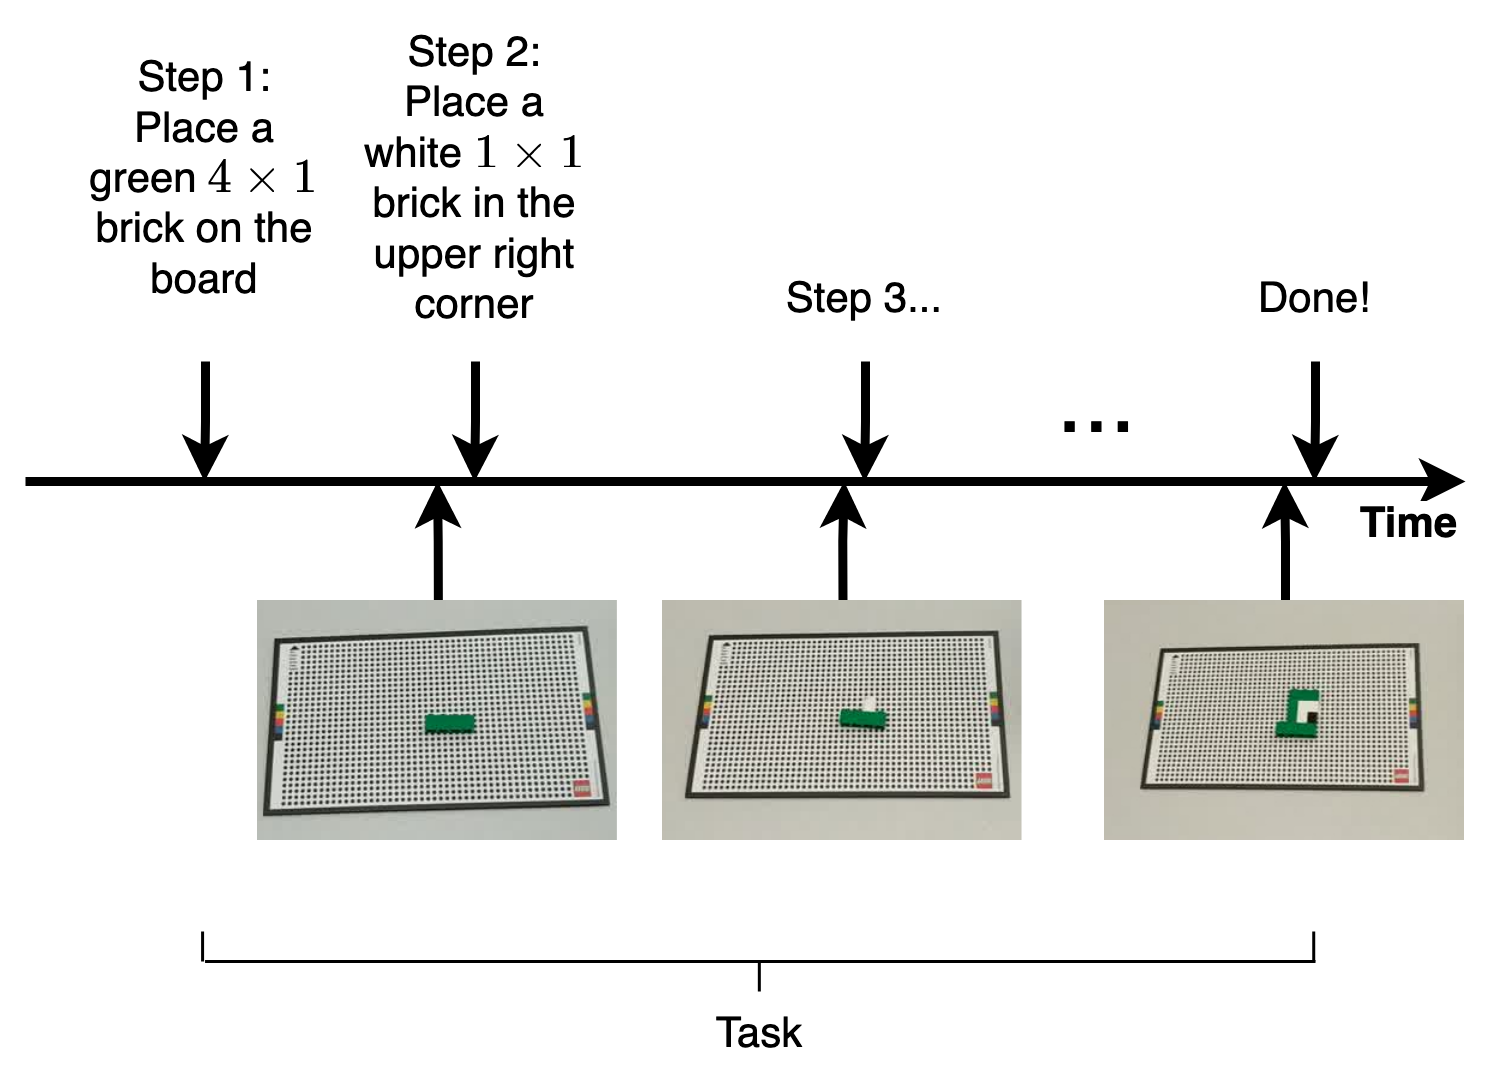
\includegraphics[width=.9\textwidth]{figs/task}
        \caption{%
            Overview of a task in a \gls{WCA}, composed of a series of steps.
            Each steps starts with an instruction being provided to the user and ends with the instruction for the next step.
            The \gls{WCA} continuously samples the task state, automatically triggering transitions between steps as correct (or incorrect) states are recognized.
        }\label{fig:task}
    \end{subfigure}\\
    \begin{subfigure}{\columnwidth}
        \centering
        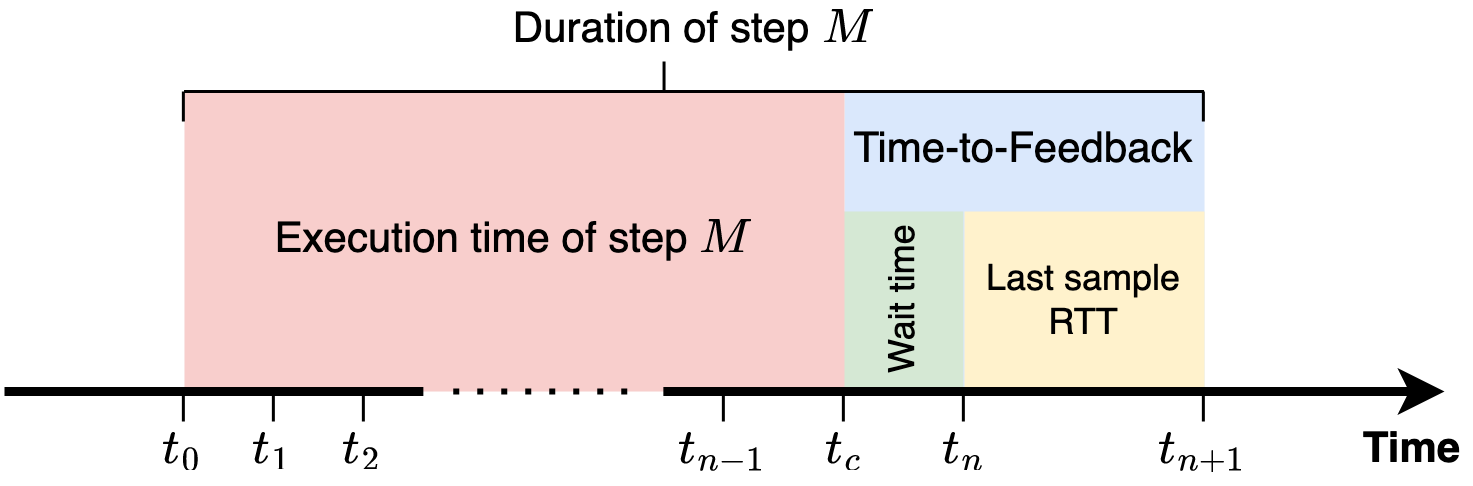
\includegraphics[width=.9\textwidth]{figs/step_time}
        \caption{%
            Breakdown of a step into its timing components.
            The instruction for step \( M \) and \( M + 1 \) are provided to the user at \( t_0 \) and \( t_{n+1} \), respectively.
            \( t_k | k \in \{1, \ldots, n \} \) correspond to the \gls{WCA} sampling instants for step \( M \), and \( t_c \) marks the instant at which the user finishes performing the instruction.
        }\label{fig:step}
    \end{subfigure}
    \caption{Key concepts in \gls{WCA}}
\end{figure}

\glsreset{WCA}

The proposed system model focuses on a specific category of novel, context-sensitive and highly-interactive \gls{MAR} applications known as \gls{WCA} applications.
We further narrow our focus on a particular sub-category --- ``step-based'' \gls{WCA} --- that have as their goal the guiding of a user through sequential tasks.
Examples of such applications are the LEGO and IKEA assistants~\cite{chen2015early,chen2018application}, in which users are guided step-by-step through the process of assembling a LEGO model and an IKEA lamp, respectively.

Step-based \glspl{WCA} operate analogously to how \gls{GPS} navigation assistants guide users, by seamlessly and continuously monitoring the progress of the user and autonomously providing relevant instructions and feedback.
The application follows the progress of the task in ``realtime'' by repeatedly sampling the state of the physical system, most commonly through video frames.
Whenever the assistant detects that the user has correctly or incorrectly performed an instruction, it provides a new instruction to either advance the task or correct the detected mistake.
The application otherwise remains silent and out-of-the-way of the user;
that is, samples which do not generate a new instruction (e.g.~because they captured an intermediate or unfinished state, or simply noise) are silently discarded.
Herein lies one of the key characteristics of these \gls{WCA} applications.
The user only consciously interacts with the application whenever they finish an instruction, and thus these are the \emph{only} points in time at which they can notice changes in system responsiveness.

To discuss these applications with precision, we provide some definitions relating to their operation.
First of all, a \emph{step} is formally understood as a specific action to be performed by the user, described by a single instruction. 
A \emph{task} consists of a series of steps to be executed in sequence (refer to \cref{fig:task}).
A step begins when the corresponding instruction is provided to the user, and ends when the instruction for the next step is provided; we call the time interval between these two events the \emph{step duration}.

\glspl{WCA} employ sampling, most commonly of video feeds, to continuously monitor the state of the real world.
Let \( \{ t_0, t_1, \ldots, t_{n + 1} \} \) represent a series of discrete and sequential sampling instants when the \gls{WCA} captures the state of the physical system, as depicted in \cref{fig:step}.
\( t_0 \) corresponds to the instant when the instruction for step \( M \) is provided and the first sample is taken,. 
\( t_n \) indicates the instant when the final sample capturing the state of \( M \) is taken. 
\( t_{n + 1} \) represents then instant when the result for sample \( t_n \) is returned and the instruction for step \( M + 1 \) is provided.

In this context, we define \( t_c \) as the point in time at which the user finishes performing the instruction for step \( M \), and the intervals \( t_c - t_0 \), \( t_n - t_c \), and \( t_{n + 1} - t_n \) as the \emph{execution time}, \emph{wait time}, and \emph{last sample \gls{RTT}}, respectively, for step \( M \).
The sum of the latter two values (i.e.\ the interval \( t_{n + 1} - t_c \)) we term \emph{\gls{TTF}}, which represents a metric used throughout this paper to describe the responsiveness of a \gls{WCA}.

% It should be noted 
% it must follow that (see also~\cite{olguinmunoz:impact2021})\footnote{\( U(a, b) \) represents the continuous uniform distribution in the open interval \( (a, b) \).}
% % \todo[inline]{I think it's an assumption rather than a must. Specifically, it is not uniform if the general execution time distribution is Rayleigh/ExpGaussian -vishnu}
% \begin{align}\label{eq:tc}
%     t_c &\thicksim U(t_{n - 1}, t_n)
% \end{align}

% Current implementations, such as those in~\cite{Chen2015LEGO,Chen2018application}, employ \emph{greedy} sampling.
% In this scheme, a new sample is immediately taken as soon as an acknowledgement is received for the previous sample.
% This means that the interval between these sampling instants is not necessarily constant, as it is subject to fluctuations due to resource contention on both the network and compute side.
% It also has as a consequence that acknowledgements must be provided even for those samples which do not cause the generation of a new instruction --- these acknowledgements are simply used for flow control and do not generate user-noticeable feedback.
\section{An optimization framework for \glsfmtshort{WCA}}

% Thus, we begin by assuming a given execution time distribution \( \mathcal{T} \), and take the modeling and partial solution approach from recents works .
% In \textcite{moothedath2021energy,moothedath2022energy1}, 

Our optimization approach focuses on the individual steps which comprise a complete \gls{WCA} task and is based on previous works on energy efficient sampling in edge-based feedback systems~\cite{moothedath2021energy,moothedath2022energy1,moothedath2022energy2}.

In~\cite{moothedath2021energy,moothedath2022energy1}, the authors model the energy in terms of the expected number of samples $\mathbb{E}[\mathcal{S}]$ and the expected wait time $\mathbb{E}[\mathcal{W}]$ experienced by the user.
They term this expression \emph{energy penalty}, and then proceed to find the optimum periodic sampling interval that minimizes it, or, equivalently, the non-constant parts of it.
Constants are excluded from this optimization, as they do not affect the process.
In particular, given that the \gls{RTT} of the final sample generally is much smaller than the total execution time of the event, it is considered part of the constants and not included in the calculation of $\mathcal{W}$.
Next, in~\cite{moothedath2022energy2}, the author retains the model and removes the constraint of periodicity to find the optimum aperiodic sampling instants $\{t_n,\,n=1,2,\dots\}$ that minimize the energy penalty.
They use a two-step approach which includes a recursive solution followed by a bisection algorithm.

In this work, we use the modeling from~\cite{moothedath2022energy2} to find the optimum aperiodic sampling interval.
However, instead of using their two-step approach, we develop a novel, approximate, but easier solution to finding the set of the optimum aperiodic sampling intervals.
Furthermore, instead of directly optimizing for energy, we expand the approach by noting that, in general, any objective metric in these applications which relates to sampling and the responsiveness of the system will present itself as a linear combination between $\mathbb{E}[\mathcal{S}]$ and $\mathbb{E}[\mathcal{W}]$ plus terms independent of the number of samples or wait time.

Let $\mathcal{E}$ correspond to such an objective metric.
Thus, 
\begin{alignat}{1}
    \Rightarrow\mathcal{E}&=\alpha\mathbb{E}[\mathcal{S}]+\beta\mathbb{E}[\mathcal{W}]+C\;\label{eq:epsilon_terminal}
\end{alignat}
% This corresponds to a Lagrangian function of this optimization, with \ensuremath{\frac{\alpha}{\beta}} representing the Lagrangian parameter.
Here, $\alpha, \beta$ and $C$ are constants responsible for modifying the objective function from one metric to another.
For instance, in the modeling used by~\cite{moothedath2021energy,moothedath2022energy1,moothedath2022energy2}, the chosen characterization results in a metric which is equal to the energy penalty.

\subsection{Finding the set of the optimum aperiodic sampling intervals}

In the following, we give the mathematical derivation of the optimum aperiodic sampling intervals.
We begin with the general solution, where the objective function to be minimized is given by \cref{eq:epsilon_terminal}.
Next, we borrow the idea of checkpointing density from~\cite{satoshi1992optimal} and define an instantaneous sampling rate function $r(t)$ such that,
\begin{alignat}{1}
{\int_{t_{n-1}}^{t_n}}r(t)\dif t=1,\;\forall n\geq1\label{eq:rt}
\end{alignat}
Note that, for periodic sampling, this function is a constant equal to the sampling frequency.
For the aperiodic case, we find $r^*(t)$, the $r(t)$ that minimizes $\mathcal{E}$.
By construction, the number of samples taken up to any time instant can be computed directly by computing the area under $r(t)$.
Thus, we obtain the expected number of samples $\mathbb{E}[\mathcal{S}]$ as
\begin{alignat}{1}
\mathbb{E}[\mathcal{S}]&=\int_{t=0}^{\infty}\bigg(\!\int_{x=0}^{t}\!\!\!\!r(x)\,\mathrm{d}x\bigg)f_{\mathcal{T}}(t)\,\mathrm{d}t\label{eq:Es}
\end{alignat}

To find  the expected wait  $\mathbb{E}[\mathcal{W}]$, we use the conditional \gls{CDF} of the execution time.
\begin{alignat}{1}
\mathbb{P}(\mathcal{W}=t_n-\mathcal{T}\leq t\,\big\vert\,t_{n-1}<\mathcal{T}\leq t_n)\nonumber\\
=\dfrac{\mathbb{P}(\mathcal{T}\geq t_n-t\,,\,t_{n-1}<\mathcal{T}\leq t_n)}{\mathbb{P}(t_{n-1}<\mathcal{T}\leq t_n)}
\end{alignat}
The numerator is degenerate when $t\!<\!0$ or $t\!>\!(t_n\!-\!t_{n-1})$.
Thus, we are only interested in $0\!\leq\!t\!\leq\! (t_n-t_{n-1})$.
Let $F_{\mathcal{T}}$, $\bar{F}_{\mathcal{T}}$ and $f_{\mathcal{T}}$ correspond to the \gls{CDF}, \gls{CCDF} and \gls{PDF} of the execution time distribution.
\begin{alignat}{1}
\!\!\!\Rightarrow\mathbb{P}(\mathcal{W}\leq t\,\big\vert\,t_{n-1}<\mathcal{T}\leq t_n)&=\dfrac{\mathbb{P}(t_n-t\leq\mathcal{T}\leq t_n)}{F_\mathcal{T}(t_n)-F_\mathcal{T}(t_{n-1})}\nonumber\\
&\approx\dfrac{F_\mathcal{T}(t_n)-F_\mathcal{T}(t_{n}-t)}{F_\mathcal{T}(t_n)-F_\mathcal{T}(t_{n-1})}\label{eq:Apx1}
\end{alignat}
Here, \cref{eq:Apx1} is an approximation merely for mathematical maturity due to the slackness of the first inequality in the numerator.
% We expand $F_\mathcal{T}(t_{n}-t)$ and $F_\mathcal{T}(t_{n-1})$ using Taylor series. Thus we can write the \gls{CCDF} as
Using Taylor series for $F_\mathcal{T}(t_{n}-t)$ and $F_\mathcal{T}(t_{n-1})$, we can express the \gls{CCDF} as
\begin{equation}
    \begin{split}
        &\begin{split}
            \Big(&F_\mathcal{T}(t_n)\\
            &-\big(F_\mathcal{T}(t_n)+f_\mathcal{T}(t_n)(-t)+\frac{f'_\mathcal{T}(t_n)(-t)^2}{2!}+\dots\big)\Big)
        \end{split}\\
        &\begin{split}
            \div
            \Big(F_\mathcal{T}(t_n)&-\big(F_\mathcal{T}(t_n)+f_\mathcal{T}(t_n)(t_{n-1}-t_n)\\
            &+\frac{f'_\mathcal{T}(t_n)(t_{n-1}-t_n)^2}{2!}+\dots\big)\Big)\label{eq:ccdf}
        \end{split}
    \end{split}
\end{equation}
Simplifying and approximating by ignoring the higher order terms, we arrive at
\begin{alignat}{1}
% &=\dfrac{F_\mathcal{T}(t_n)-\big(F_\mathcal{T}(t_n)+f_\mathcal{T}(t_n)(-t)+f'_\mathcal{T}(t_n)(-t)^2/2!+\dots\big)}{F_\mathcal{T}(t_n)-\big(F_\mathcal{T}(t_n)+f_\mathcal{T}(t_n)(t_{n-1}-t_n)+f'_\mathcal{T}(t_n)(t_{n-1}-t_n)^2/2!+\dots\big)}\\&
\mathbb{P}(\mathcal{W}\leq t\,\big\vert\,t_{n-1}<\mathcal{T}\leq t_n)&\approx\dfrac{tf_\mathcal{T}(t_n)}{(t_{n}-t_{n-1})f_\mathcal{T}(t_n)}\label{eq:Apx2}\\
\Rightarrow\mathbb{P}(\mathcal{W}> t\,|\,t_{n-1}<\mathcal{T}\leq t_n)&= 1-\dfrac{t}{(t_{n}-t_{n-1})}\nonumber
\end{alignat}

Next, using the expression for the \gls{CCDF} in \cref{eq:ccdf}, we find the conditional expectation of $\mathcal{W}$.
\begin{alignat*}{1}
% \mathbb{P}(\mathcal{W}> t\,|\,t_{n-1}<\mathcal{T}\leq t_n)&\approx 1-\dfrac{t}{(t_{n}-t_{n-1})}\\
\Rightarrow \mathbb{E}[\mathcal{W}\,|\,t_{n-1}<\mathcal{T}\leq t_n]&=\smashoperator[r]{\int_{0}^{t_n-t_{n-1}}}\Big(1-\dfrac{t}{(t_{n}-t_{n-1})}\Big)\,\mathrm{d}t\\
&=\dfrac{(t_n-t_{n-1})}{2}.
\end{alignat*}
% However, we can also approximate $(t_n-t_{n-1})$, the sampling interval to the inverse of the instantaneous sampling frequency $r(t)$. This approximation (\ref{Apx3}) is valid as long as $r(t)$ is varying slowly between two consecutive sampling instants. That is,
If $r(t)$ is varying slowly between two consecutive sampling instants due to the closeness of two sampling intervals, we can approximate the sampling interval $(t_n\!-\!t_{n-1})$ as
\begin{alignat}{1}
 (t_n-t_{n-1})&\approx\dfrac{1}{r(t)},\;\forall t,n:t_{n-1}\!<\!t\!\leq\!t_n.\label{eq:Apx3}\\
% \end{alignat}
% As a result, we can compute the expected wait as,
% \begin{alignat}{1}
\Rightarrow \mathbb{E}[\mathcal{W}]&=\int_{0}^{\infty}\mathbb{E}[\mathcal{W}\,|\,t_{n-1}<\mathcal{T}\leq t_n]f_\mathcal{T}(t)\,\mathrm{d}t\nonumber\\
&=\int_{0}^{\infty}\dfrac{1}{2r(t)}f_\mathcal{T}(t)\,\mathrm{d}t.\label{eq:Ew}
\end{alignat}
We can thus find the energy penalty using \cref{eq:Es} and \cref{eq:Ew} as
\begin{alignat*}{1}
\mathcal{E}&=\int_{0}^{\infty}\Big(\alpha\int_{x=0}^{t}r(x)\,\mathrm{d}x+\beta\dfrac{1}{2r(t)}\Big)f_{\mathcal{T}}(t)\,\mathrm{d}t.\label{eq:epsilon_eulerForm}\\
\intertext{%
    Let $g(t)=\int_{0}^{t}r(x)\dif x$.
    Then  $g'(t)=\tfrac{\mathrm{d}}{\mathrm{d}t}g(t)=r(t)$.
    That is,
}
\mathcal{E}&=\int_{0}^{\infty}\Big(\alpha g(t)+\dfrac{\beta}{2g'(t)}\Big)f_{\mathcal{T}}(t)\,\mathrm{d}t
\end{alignat*}

As per the Euler-Lagrange equation from the calculus of variations~\cite{bellman1954dynamic,arfken2013calculus}, the extreme value of $\mathcal{E}$ is obtained at
\begin{alignat}{1}
r^*(t)&=\sqrt{\dfrac{\beta f_\mathcal{T}(t)}{2\alpha\bar{F}_\mathcal{T}(t)}}.\\
\intertext{Thus, for a Rayleigh distributed $\mathcal{T}$ with parameter $\sigma$,}
r^*(t)&=\sqrt{\dfrac{\beta t}{2\alpha\sigma^2}}\\
\Rightarrow &\int_{t_n}^{t_{n+1}}\!\!\!\sqrt{\dfrac{\beta t}{2\alpha\sigma^2}}\,\mathrm{d}t=1,\;\forall n\geq1\nonumber\tag{from \eqref{eq:rt}}\\
\Rightarrow &\;t_{n+1}^{\frac{3}{2}}-t_{n}^{\frac{3}{2}}=3\sigma\!\sqrt{\tfrac{\alpha}{2\beta}}\nonumber\\
\intertext{We have $t_0=0$. Substituting $n=1,2,\dots$, in order, in the above equation provides us our final result}
&\;t_n=\Big(3\sigma\!\sqrt{\tfrac{\alpha}{2\beta}}\Big)^{\frac{2}{3}}n^{\frac{2}{3}}\;\blacksquare\label{eq:tnRayleigh}
\end{alignat}

% Note that throughout the paper we use a exGaussian distribution but not Rayleigh. This is because, 
% Note that, due to the close similarity in their density functions, the task times can be approximated fairly equally to an \gls{exGaussian} distribution as well as a Rayleigh distribution, with the former attracting more attention from works like~\cite{rohrer1994analysis,palmer2011what,marmolejo_ramos2022generalised}.
% This is the reason why the above results are applicable in this work where we have predominantly considered \gls{exGaussian} distribution.
% Furthermore, we have also verified the closeness of the results as well as the validity of the approximations made in the proofs using distribution fitting and simulations.

\subsubsection{Optimizing for expected number of samples}

We first look at the application of \cref{eq:epsilon_terminal} and its solution in \cref{eq:tnRayleigh} to the optimization of number of captured samples per step.
We start with this metric as its implications for resource consumption and responsiveness are straightforward to understand.
On the one hand, higher sampling rates directly lead to perceived increased system responsiveness, as smaller sampling intervals translate into smaller maximum wait times.
On the other, the relationship between number of samples captured and sent and network congestion is generally understood to be exponential-like, and too high sampling rates quickly lead to bottlenecks on the network, particularly in multi-tenant environments.
Additionally, the energy cost of capturing a sample on a \gls{WCA} client device is often much higher than remaining in an idle state, and thus excessive sampling leads to drastically increased energy consumption.
Optimizing the number of samples captured per step can thus be a straightforward way of reducing resource consumption and contention in \gls{WCA} applications.

However, an unconstrained optimization of the number of samples is trivial and meaningless as the solution points to a single sample at $t\!\rightarrow\!\infty$, taking the wait time to infinity.
Thus, we look at the constrained optimization of the expected number of samples with an upper bound $w_0$ for the expected wait.
That is, $\mathbb{E}[\mathcal{W}]\!\leq\!w_0$.

First note that the general solution has constants $\alpha$ and $\beta$ corresponding to the weights given to the cost of sampling and waiting, respectively.
The optimization criteria changes from minimizing wait time to minimizing the number of samples when the ratio $\frac{\alpha}{\beta}$ goes from zero to infinity.
Since any positive real value is valid for this ratio, one can achieve any valid points $(\mathbb{E}[\mathcal{S}],\mathbb{E}[\mathcal{W}])$ via simply by varying the ratio $\frac{\alpha}{\beta}$.

Furthermore, since the sampling instants are aperiodic and can take any positive real values, the bound will be tight at the optimum. 
% This is because (1) a higher bound on $\mathbb{\mathcal{W}}$ is always associated with a lower optimum on $\mathbb{\mathcal{S}}$ and (2) any $\mathbb{\mathcal{W}}$ can be achieved, for instance by a scaling all the sampling instance of a given policy by an appropriate constant.
Hence, to solve for the modified optimization problem that minimizes $\mathbb{E}[\mathcal{S}]$ with an upper bound $w_0$ on $\mathbb{E}[\mathcal{W}]$, we equate \cref{eq:Ew} to $w_0$, find the corresponding $\frac{\alpha}{\beta}$, and find the optimum set of sampling instants by plugging this ratio into \cref{eq:tnRayleigh}.
\begin{alignat*}{1}
\mathbb{E}[\mathcal{W}]&=\int_{0}^{\infty}\dfrac{1}{2r(t)}f_\mathcal{T}(t)\,\mathrm{d}t.\nonumber\\
&=\int_{0}^{\infty}\frac{1}{2}\sqrt{\frac{2\alpha\sigma^2}{\beta t}}\cdot \frac{t}{\sigma^2}e^{-{t^2}/{2\sigma^2}}\mathrm{d}t\\
&=\sqrt{\frac{\alpha\sigma^2}{2\beta}}\int_{0}^{\infty}\frac{\sqrt{t}}{\sigma^2}e^{-{t^2}/{2\sigma^2}}\mathrm{d}t\\
&=\sqrt{\frac{\alpha\sigma^2}{2\beta}}\left({\frac{1}{{2}\sigma^2}}\right)^{1/4}\cdot\int_{0}^{\infty}y^{-1/4}e^{-y}\mathrm{d}y\\
&=\sqrt{\frac{\alpha\sigma^2}{2\beta}}\left({\frac{1}{{2}\sigma^2}}\right)^{1/4}\cdot\mathlarger{\Gamma}(\tfrac{3}{4}),\\
% &\approx 0.728637\sqrt{\frac{\alpha\sigma}{\beta}}\\
\intertext{%
    where $\mathlarger{\Gamma(x)}$ is the gamma function.
    Thus, when the upper bound $w_0$ is tight,
}
\mathbb{E}[\mathcal{W}]&=w_0=\sqrt{\frac{\alpha\sigma}{2\sqrt{2}\beta}}\mathlarger{\Gamma}(\tfrac{3}{4})\\
\Rightarrow\frac{\alpha}{\beta}&=\frac{w_0^2}{\sigma}\frac{2\sqrt{2}}{(\mathlarger{\Gamma}(\tfrac{3}{4}))^2}\\
% &=1.88355\frac{w_0^2}{\sigma}
&\approx1.9\frac{w_0^2}{\sigma}.
\end{alignat*}
Plugging this into \cref{eq:tnRayleigh}, leaves us with the following expression for the optimal aperiodic sampling intervals when optimizing for number of samples
\begin{alignat}{1}
    t_n&=\Big(3\sigma\!\sqrt{\tfrac{\alpha}{2\beta}}\Big)^{\frac{2}{3}}n^{\frac{2}{3}}\nonumber\\
    &=\Big(3\sigma\!\sqrt{\tfrac{1.9w_0^2}{2\sigma} }\Big)^{\frac{2}{3}}n^{\frac{2}{3}}\;\blacksquare\label{eq:tnRayleigh:samples}
\end{alignat}

\subsubsection{Optimizing for energy consumption}

Next we will look at the application of this framework to the direct optimization of expected energy consumption.
Although, as mentioned above, minimizing the number of samples captured during a step can potentially translate into a reduction in the energy consumption, this is not a given.
Energy consumption depends on multiple other factors other than number of samples captured, such as idle versus communication power and delays, and thus cannot be optimized by simply minimizing the number of samples taken.

In the following, we take the general solution, \cref{eq:epsilon_terminal}, and find the appropriate \( \alpha \) and \( \beta \) to minimize the energy consumed per step, i.e.\ \( \mathcal{E}=E \).
We directly take the modeling from~\cite{moothedath2022energy2} with a necessary modification in the assumption of one-way communication in all but the final sample.
With feedback given even to the discarded samples in our model and communication delay defined as the total delay in either direction, we have, 
\begin{alignat}{2}
    \mathrm{E}=&\;\mathcal{S}\tau_cP_c+(\mathcal{T}+\mathcal{W}+\tau_\mathrm{p}+\tau_\mathrm{c}-\mathcal{S}\tau_c)P_0\nonumber\\
    % &=s\tau_c(P_c-P_0^{(t)})+wP_0^{(t)}+(\tau+\tau_c+\tau_p) P_0^{(t)}+\tau_cP_c\\
    =&\;\tau_{\text{c}}(P_{\text{c}} -P_0)\mathcal{S}+\mathcal{W}P_0+(\mathcal{T}+\tau_{\text{p}} +\tau_{\text{c}}) P_0\nonumber\\
&\Rightarrow \alpha=\tau_{\text{c}}(P_{\text{c}} -P_0),\text{ and }\beta=P_0 \label{eq:optimization:energy}
\end{alignat}
\( \tau_\text{p} \) and \( \tau_\text{c} \) correspond to the processing and two-way communication delay for each sample.
\( P_\text{c} \) and \( P_0 \) correspond to the communication and idle power, respectively, of the \gls{WCA} client device.

Plugging then \cref{eq:optimization:energy} into \cref{eq:tnRayleigh}, gives us the final expression for the optimum sampling intervals when optimizing for energy consumption,
\begin{alignat}{1}
    t_n&=\Big(3\sigma\!\sqrt{\tfrac{\alpha}{2\beta}}\Big)^{\frac{2}{3}}n^{\frac{2}{3}}\nonumber\\
    &=\Big(3\sigma\!\sqrt{\tfrac{\tau_{\text{c}}(P_{\text{c}} -P_0)}{2 P_0}}\Big)^{\frac{2}{3}}n^{\frac{2}{3}}\;\blacksquare\label{eq:tnRayleigh:energy}
\end{alignat}

\subsection{Comparison with exact solution}

\todo[inline]{TODO}

\subsection{Implementation}

\todo[inline]{TODO: what to put here?}
\section{A model of human behavior for \gls{WCA}}\label{sec:model}

\todo[inline]{Rewrite!}

In the following, we employ the above insights together with the data collected for~\cite{olguinmunoz2021impact} to design and build a probabilistic model of human behavior for \gls{WCA}.
We detail the construction of a model which uses the data collected to generate, at runtime, realistic execution times. 
In order to accurately emulate the behavior of a human, such a model needs to implement two main behaviors.
First, it needs to generate realistic execution times for each step in the task, considering the current and historical impairment of the \gls{WCA} system, as well as salient individual-difference measures.
We detail this in \cref{ssec:model:exectimes}.
Neuroticism is incorporated in this aspect of the model, as it is the most salient individual difference in the data;
however, other factors such as immersive tendency could be treated similarly.
Second, the model must produce sequences of input samples for each step mimicking what a real human would generate; this is explained in \cref{ssec:model:frames}. 
% Finally, in \cref{ssec:model:obtaining} we briefly discuss where implementations of this model can be obtained.


\subsection{Generating realistic execution times}\label{ssec:model:exectimes}

% As expressed in \cref{ssec:plos}, for \textcite{olguinmunoz:impact2021} we collected timing and task performance data for \num{40} participants performing a \num{169}-step task, guided by a \gls{WCA}, as well as personality trait scores for each participant.
% For this paper, we use this data to construct a probabilistic model for the generation of realistic execution times.
The processing of the data from~\cite{olguinmunoz2021impact} for the generation of execution times can be summarized as a grouping according to discretized levels of neuroticism and a weighted rolling average of \gls{TTF}.
The resulting collections of execution times represent the distributions of these values for users with specific levels of neuroticism, interacting with systems at specific states of impairment and recent histories of impairment.
These distributions can then be sampled to produce new, realistic execution times.
In the following, we detail the step-by-step processing of this data and construction of the probabilistic model.

We employ a cleaned and re-parameterized copy of the timing data.
The \num{6760} data points are arranged in a table together with identifiers for the subjects, their normalized neuroticism score, and a sequence number for each step.

\begin{table*}[]
    \centering
    \caption{%
        Default bins used for model parameter levels.
        Values have been rounded to two decimal places.
    }
    \label{tab:defaultbins}
    \begin{tabular}{@{}lccccccc@{}}
        \toprule
        \textbf{Parameter} & \textbf{Low} & & & \textbf{Medium} & & & \textbf{High}         \\ \midrule
        Neuroticism        & \( [0, 0.5) \) & & & & & & \( [0.5, 1.0] \)      \\
        Weighted TTF & \([0.0], 0.82]\) & \((0.82, 1.53]\) & \((1.53, 2.08]\) & \((2.08, 2.67]\) & \((2.67, 3.45]\) & \((3.45, 4.13]\) & \((4.13, \infty]\)
    \end{tabular}
\end{table*}

We begin by calculating rolling weighted averages of the \glspl{TTF} of each of the \num{40} individual repetitions of the data.
We use exponentially decaying weights for the most recent \num{12} steps, defined in \cref{eq:weights}, such that the most recent \gls{TTF} accounts for roughly \SI{50}{\percent} of the rolling average, the second-most recent for \textasciitilde\SI{25}{\percent}, the third-most \textasciitilde\SI{12}{\percent}, and so on.
We additionally pad the data for each run with \num{12} copies of the first \gls{TTF} in order to ensure sensible values for the first twelve steps; this padding is removed after the weighted values have been calculated.
This weighing ensures that drastic changes in \gls{TTF} are significantly remembered by the model for at least \num{4} steps --- in line with our previous findings on human behavior --- and are subsequently quickly forgotten.
\begin{equation}\label{eq:weights}
    w_{n - i} = 
    \left\{ \begin{array}{ll}
        \frac{e^{-0.7 i}}{\sum\limits^{12}_{j=1} e^{-0.7 j}} & 1 \leq i \leq 12 \\
        & \\
        0 & i > 12
    \end{array} \right.
\end{equation}

The resulting weighted \glspl{TTF} are then binned into continuous ranges by splitting the data on the \num{7}-quantiles.
The exact resulting bins of this operation on the data are presented in \cref{tab:defaultbins}.

Next, the data is further tagged according to its associated level of normalized neuroticism.
For this work, we use two levels, \emph{low} and \emph{high}, the exact values for which can also be seen in \cref{tab:defaultbins}.

After this preprocessing has been finished, the data is ready to be used for the generation of execution times by applying the above steps in real-time to measured \glspl{TTF}:

\begin{enumerate}
    \item At the beginning of each step, the model is fed the measured \gls{TTF} for the previous step.
    \item The model calculates a weighted average over the latest \num{12} steps using the weights defined in \cref{eq:weights}.
    \item The resulting weighted \gls{TTF} is binned into the corresponding range (\cref{tab:defaultbins}).
    \item The model then filters the pre-processed data to find execution time samples associated with this same discretized weighted \gls{TTF}.
    \item The selected samples are further filtered to match the desired level of neuroticism.
    \item The remaining samples are then used to output a realistic execution time, either by
    \begin{itemize}
        \item directly sampling the execution time values;
        \item or, using \gls{MLE} to fit a distribution to the execution time samples and then sampling the distribution instead.
    \end{itemize}
\end{enumerate}

The distribution chosen for the second variant described above corresponds to the \gls{exGaussian} distribution, previously discussed in \cref{ssec:moderationeffects}.

We implement these two variants of the model in Python 3.10, and verify their correct behavior in the following.

\subsubsection{Verifying the behavior of the timing model}\label{ssec:model:verification}
% \todo[inline]{Based on the 4 main conclusions of the PLOS paper.}

We verify the behavior of the above described model with respect to the four main conclusions of our work in~\cite{olguinmunoz2021impact}, which were previously discussed in \cref{ssec:plos}.
These are reformulated as objectives below:

\begin{enumerate}
    \item\label{it:ttftoexectime} Higher \glspl{TTF} should result in higher execution times.
    \item\label{it:duration} When subject to a series of steps at the same level of impairment, desired behavior depends on the level:
    \begin{enumerate}
        \item At low \glspl{TTF}, the model should speed up; i.e.\ execution times should decrease.
        \item At medium \glspl{TTF}, execution times should remain more or less the same.
        \item At high \glspl{TTF}, execution times should increase.
    \end{enumerate}
    \item The effects on execution times due to past changes in system responsiveness should linger for at least a few steps whenever system responsiveness changes anew.
    \item\label{it:neuro} Finally, neuroticism should act as a modulating factor for the above effects.
\end{enumerate}

\begin{figure}
    \centering
    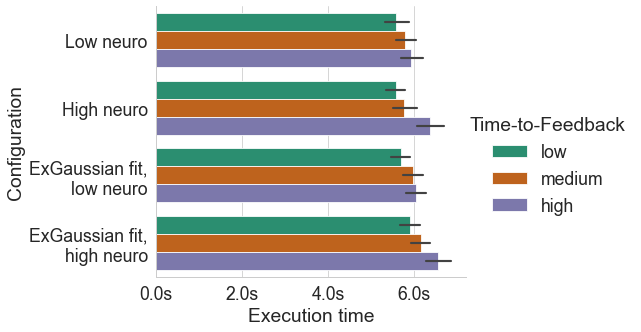
\includegraphics[width=\textwidth]{figs/new_model/ttf_to_exectime}
    \caption{%
        Effects of feeding three different \glspl{TTF} (\emph{low}, \SI{0}{\second}, \emph{medium}, \SI{2.5}{\second}, or \emph{high}, \SI{5}{\second}) into the model on the generated execution times.
        Higher \glspl{TTF} directly lead to higher execution times.
        Error bars indicate the \SI{95}{\percent} \gls{CI}.
    }\label{fig:ttf_to_exectime}
\end{figure}

\cref{fig:ttf_to_exectime} shows the mean execution time outputted by the model when fed three different levels of \gls{TTF} (\emph{low}, \SI{0}{\second}, \emph{medium}, \SI{2.5}{\second}, or \emph{high}, \SI{5}{\second}).
These results were generated by first warming up the model by feeding it \num{25} \glspl{TTF} selected at random from the data before feeding it the desired input \gls{TTF}, and recording the generated execution time.
This procedure is repeated \num{600} times for each configuration and target \gls{TTF}.
The resulting mean execution times match precisely the desired behavior mentioned in \cref{it:ttftoexectime}, with the difference in mean execution times at low versus high \glspl{TTF} reaching \SI{14}{\percent} (\textasciitilde\SI{5.6}{\second} to \textasciitilde\SI{6.4}{\second}) in the worst case (high neuroticism configuration).
Additionally, we can observe the effects of neuroticism on generated execution times, as specified in \cref{it:neuro}.
At low neuroticism, the average difference between execution times at low versus high \glspl{TTF} was of roughly \SI{6.2}{\percent}, compared to \SI{12.5}{\percent} at high neuroticism.

\begin{figure}
    \centering
    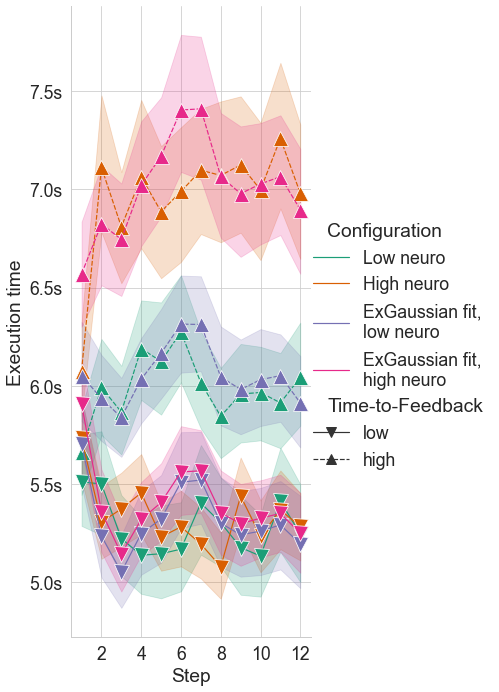
\includegraphics[height=25em]{figs/new_model/exectime_over_steps}
    \caption{%
    Effects of prolonged exposure to constant levels of system impairment on the model.
    At low (\SI{0}{\second}) \gls{TTF}, the models speed-up over time; conversely at high (\SI{5.0}{\second}) \gls{TTF}, the models either present no change or drastically increase their generated execution times, depending on the level of neuroticism.
    Error bands indicate \SI{95}{\percent} \gls{CI}.
    }\label{fig:exectimeduration}
\end{figure}

Next, \cref{fig:exectimeduration} shows the evolution of generated execution times while the model is subject to a fixed \gls{TTF}, either \emph{low} (\SI{0}{\second}) or \emph{high} (\SI{5}{\second}).
These results were generated by first warming up the model with \num{25} random \glspl{TTF}, and then recording the generated execution times over a sequence of \num{12} steps at a fixed \gls{TTF}; this procedure is repeated \num{600} times for each configuration and target \gls{TTF}.
Once again, we see here behavior matching what is expected of the model, in particular with respect to \cref{it:duration}.
At low \glspl{TTF}, the model is on average, across all configurations, \SI{8.2}{\percent} faster at step \num{12} when compared to step \num{1}.
At high \glspl{TTF}, the behavior changes depending on the level of neuroticism of the model.
Low neuroticism models basically do not change their execution times, whereas high neuroticism configurations are on average \SI{10}{\percent} slower after \num{12} steps.
This is once again in line with our previous findings, as we had previously concluded that humans tend to speed up during a task, but that this speed-up is hindered and eventually reversed as system responsiveness decreases, and that the strength of this effect is correlated with neuroticism.

\begin{figure*}
    \centering
    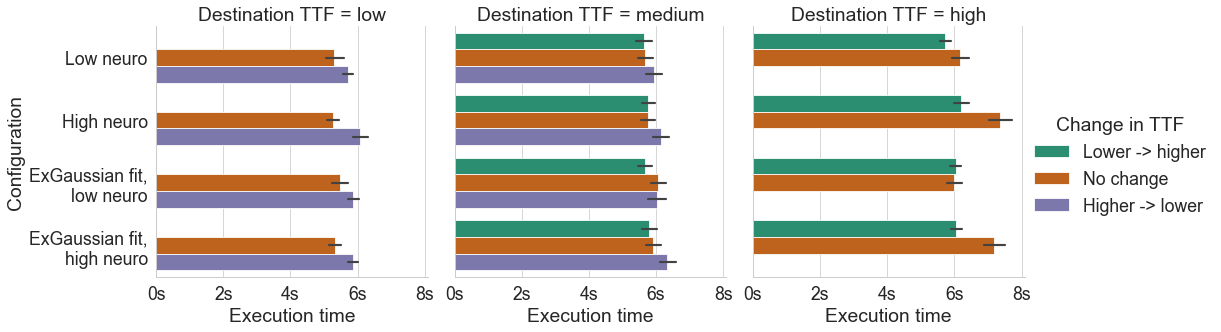
\includegraphics[width=\textwidth]{figs/new_model/transitions}
    \caption{%
        Effects of changes in system impairment on subsequently generated execution times.
        These effects linger on after the change, and thus execution times immediately after a transition are either consistently lower or higher than otherwise at the new \gls{TTF}, depending on the old \gls{TTF}.
        Error bars indicate \SI{95}{\percent} \gls{CI}.
    }\label{fig:transitions}
\end{figure*}

Finally, in \cref{fig:transitions} we showcase the behavior of the model when comparing execution times generated immediately after a change in system responsiveness.
We generate these results by first warming up the model by feeding it a fixed \gls{TTF} (which we will refer to as the \emph{origin} \gls{TTF}) \num{25} times.
Next, another \gls{TTF} value (the \emph{destination} \gls{TTF}) is fed to the model, and we record the output execution time.
Each sample is tagged according to the relation between origin and destination \gls{TTF}, either lower to higher, higher to lower, or equal.
As before, we run \num{600} repetitions of this procedure for each combination of model configuration, origin \gls{TTF}, and destination \gls{TTF}.
Execution times generated immediately after a transition from a higher \gls{TTF} into a lower one are consistently higher than execution times generated without a preceding change in \glspl{TTF}.
Conversely, execution times are consistently lower than otherwise immediately after a change from a lower \gls{TTF} into a higher one.
These results are once again in line with our findings in~\cite{olguinmunoz2021impact}, in which we found lingering effects of transitions between levels of system impairment on human execution times.


\subsection{Generating realistic samples}\label{ssec:model:frames}

Apart from the aforementioned timing and performance data, for~\cite{olguinmunoz2021impact} we also recorded all collected video frame samples together with matching metadata.
For each video frame submitted to the \gls{WCA} during the tasks, we recorded
\begin{inlineenum}
    \item the raw video frame captured
    \item sample submission timestamp
    \item \gls{WCA} processing completed timestamp
    \item result or acknowledgement returned timestamp
    \item a tag representing the result of the \gls{WCA} processing
\end{inlineenum}.
The tags assigned corresponded to:
\begin{description}[font={\bfseries\ttfamily}, wide]
    \item[SUCCESS:] frames which triggered a transition to a new step (or the correction of a previous mistake) in the logical task model of the \gls{WCA}, and thus cause the generation of feedback to the user.
    \item[REPEAT:] frames which captured the same board state as the previous successful frame, and thus produced no feedback.
    \item[LOW\_CONFIDENCE] frames for which the image recognition algorithm in the \gls{WCA} did not reach the necessary confidence threshold to interpret it as a valid board state.
        These frames also produce no feedback.
    \item[BLANK] frames in which not enough of the board is visible due to noise, movement, occlusion, etc.
        These frames produce no feedback either.
    \item[TASK\_ERROR] frames which contained an incorrect board state and thus triggered a transition to a procedural corrective step and the generation of feedback to the user.
        However, it must be noted that none of the \num{40} participants made any mistakes during the task, and thus no such frames were encountered in the data.
\end{description}

We correlate this frame data with the step timing data described in \cref{ssec:model:exectimes} to match frames with their corresponding step execution times.
We assign to each frame a normalized instant value \( t_\text{norm} \) corresponding to its capture instant \( \tau \) (expressed in seconds since the start of the step) divided by the total execution time \( t_\text{exec} \) of the step:

\begin{align}
    \left( t_\text{norm} = \frac{\tau}{t_\text{exec}} \right) \in [0, 1]\label{eq:tnorm}
\end{align}

% To exemplify, for a step with execution time \( t_\text{exec} = \SI{10}{\second} \), a frame captured at time \( \tau = \SI{3}{\second} \) from the start of the step, will have a normalized instant value \( t_\text{norm} \):
% \begin{align}
%     t_\text{norm} = \frac{\tau}{t_\text{exec}} = \frac{\SI{3}{\second}}{\SI{10}{\second}} = 0.3
% \end{align}

This allows us to analyze the distribution of frame tag probabilities as a step progresses, independently of execution times.
This is illustrated in \cref{fig:frameprobs}.
Intuitively, \texttt{REPEAT} frames dominate the early instants after a step transition, as the user has not had time to start performing the new instruction and thus the \gls{WCA} keeps capturing frames representing the previous state of the board.
As the user starts moving and performing actions, \texttt{BLANK} frames start to dominate, as this activity prevents the \gls{WCA} from capturing ``clean'' frames.
Finally, it must be noted that \texttt{SUCCESS} frames are not included in this probability density plot, as, by definition:
\begin{equation}
    P(\text{\texttt{SUCCESS}} | t_\text{norm}) =
    \left\{ \begin{array}{ll}
        0 & t_\text{norm} < 1.0    \\
        1 & t_\text{norm} \geq 1.0
    \end{array} \right.
\end{equation}

That is, any frame captured immediately at or after the execution time has been reached will contain the finished board state and thus correspond to a \texttt{SUCCESS} frame.

\begin{figure}
    \centering
    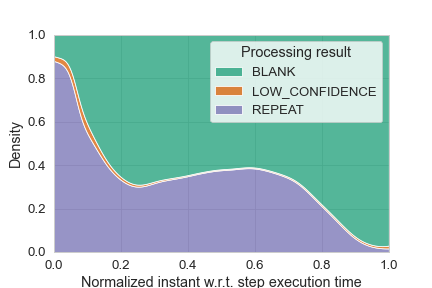
\includegraphics[width=.9\textwidth]{model_data/frame_probabilities}
    \caption{%
        Probability density of frame result tags as a step progresses.
        Note that \texttt{SUCCESS} frames are not included as --- by definition --- the probability for success frames is \num{1} for all normalized instant values greater than or equal to \num{1.0}.
    }\label{fig:frameprobs}
\end{figure}

Using the above insights, together with the corresponding recorded video frames, we devise a scheme for the procedural generation of a synthetic trace for any step in \gls{WCA} task in the same category as those used in~\cite{olguinmunoz2021impact}.
We first prepare a discretized representation of the probability density map in \cref{fig:frameprobs}.
We segment the normalized instant value into a number of discrete bins (\num{25} in this work), and calculate the relative fraction of frames for each category in each bin.
For each step, given
\begin{inlineenum}
    \item a collection of random non-\texttt{SUCCESS}, non-\texttt{REPEAT} frames (at least one frame for each of the \texttt{BLANK} and \texttt{LOW\_CONFIDENCE} categories)
    \item an appropriate \texttt{SUCCESS} video frame containing the correct state for the step
    \item an appropriate \texttt{REPEAT} video frame containing the correct state for the \emph{previous} step
\end{inlineenum},
we can then procedurally generate a trace by randomly selecting appropriate frames according to the distributions presented in \cref{fig:frameprobs}.
In other words, for each sampling instant in a step with a given execution time \( t_\text{exec} \):
\begin{enumerate}
    \item We calculate \( t_\text{norm} \) according to \cref{eq:tnorm}.
    \item If \( t_\text{norm} \ge 1.0 \), we select the \texttt{SUCCESS} frame and stop sampling.
    \item If instead \( t_\text{norm} < 1.0 \), we find the appropriate bin for \( t_\text{norm} \) and then select a frame by performing a weighted random sampling of the frame categories in the normalized instant bin.
\end{enumerate}

\subsection{Obtaining the model}\label{ssec:model:obtaining}

We provide the model implementations in Python~\num{3.10} as well as the base data to the community as \gls{FOSS}.
All of these are published on the \href{https://github.com/KTH-EXPECA/EdgeDroid2}{\texttt{KTH-EXPECA/EdgeDroid2}} repository on GitHub under a permissive Apache version 2 license.

\section{Results}

\subsection{Optimizing for mean number of samples per step}\label{ssec:optimization:samples}

We first look at the application of \cref{eq:epsilon_terminal} for the optimization of number of captured samples per step.
We start with this metric as its implications for resource consumption and responsiveness are straightforward to understand.
On the one hand, higher sampling rates directly lead to perceived increased system responsiveness, as smaller sampling intervals translate into smaller maximum wait times.
On the other, the relationship between number of samples captured and sent and network congestion is exponential, and too high sampling rates quickly lead to bottlenecks on the network, particularly in multi-tenant environments.
Additionally, the energy cost of capturing a sample on a \gls{WCA} client device is often much higher than remaining in an idle state, and thus excessive sampling leads to drastically increased energy consumption.
Optimizing the number of samples captured per step can thus be a straightforward way of reducing resource consumption and contention in \gls{WCA} applications.

However, an unconstrained optimization of the number of samples is trivial and meaningless as the solution points to a single sample at $t\!\rightarrow\!\infty$, which also takes the wait time to infinity.
Thus, we look at the constrained optimization of the expected number of samples with an upper bound $w_0$ for the expected wait.
That is, $\mathbb{E}[\mathcal{W}]\!\leq\!w_0$.
We show in \cref{appx1} that we can find appropriate $\alpha$ and $\beta$ for this problem by satisfying the condition
\begin{alignat}{1}\label{eq:optimization:sampling}
\frac{\alpha}{\beta}=\frac{2\sqrt{2}\,w_0^2}{(\mathlarger{\Gamma}(\tfrac{3}{4}))^2\,\sigma}\approx1.9\frac{w_0^2}{\sigma}
\end{alignat}
where $\mathlarger{\Gamma}(x)$ is the Gamma function.

\medskip

We introduce here a reference scheme to which we will compare our approach.
In~\cite{wang2019towards}, \citeauthor{wang2019towards} introduce an adaptive sampling scheme for \gls{WCA} intended to reduce the number of samples processed per step while still meeting application responsiveness bounds.
At every sampling instant \( t \), the scheme adapts the sampling rate \( R(t) \) of the system according to the estimated likelihood of the user having finished the step,
following the formula 

\begin{equation}
    R(t) = R_\text{min} + \varphi\left( R_\text{max} - R_\text{min} \right) * CDF(t)
\end{equation}

\( R_\text{max} \) and \( R_\text{min} \) correspond to the maximum and minimum sampling rates of the system, respectively.
\( R_\text{max} \) can directly be assumed to correspond to \( 1 / \text{\gls{RTT}}_\mu \), where \( \text{\gls{RTT}}_\mu \) corresponds to the mean \gls{RTT} of the system.
\( R_\text{min} \) needs to either be calculated according to the latency bounds of the system or specified manually.
\( \varphi \) corresponds to a scaling factor and \( t \) to the time of the current sampling instant with respect to the start of the step.
Finally, \( CDF \) corresponds to the \gls{CDF} of a distribution describing the execution times for the current step; \citeauthor{wang2019towards} used a single static Gaussian distribution for all steps in their work.

\medskip

In the following, we will show the effects of our optimization approach combined with our timing models compared to the state-of-the-art approach~\cite{wang2019towards}.
For this we implement these sampling schemes in Python and run a number of simulations with them.
The first scheme uses our approach, \cref{eq:epsilon_terminal,eq:optimization:sampling}, to determine the optimum sampling instants and the values for \( \alpha \) and \( \beta \) at each step.
It includes an embedded timing model (without any distribution fitting) to provide updated estimates of the mean execution time \( \mu \) and \( \sigma \) at every step as well, allowing it to adapt to the state of the system.
We will refer to this scheme as the \emph{sample-count-optimized aperiodic} sampling scheme.

We implement \citeauthor{wang2019towards}'s original design using a Gaussian distribution fitted to all the execution times collected for~\cite{olguinmunoz2021impact} for \gls{CDF} calculation.
This scheme does not include an embedded timing model, and uses the same \gls{CDF} for every step.

Finally, we also implement two reference sampling schemes representing best- and worst-case extremes.
The first of these corresponds to the offline optimum which uses an embedded \emph{oracle} to perfectly predict the execution time of each step.
Such an ideal scheme is thus able to always sample exactly once per step, with a constant wait time of zero.
The second reference scheme corresponds to one which \emph{greedily} samples as much as possible.
This represents a completely unoptimized design with no considerations for resource-consumption trade-offs; it simply attempts to maximize the number of captured samples per step.
This is an interesting approach to include as it corresponds to the sampling strategy used in most existing \gls{WCA} prototypes.

\begin{table}
    \centering
    \caption{Experimental parameters}\label{tab:params}
    \begin{tabular}{lrl}
        \toprule
        Parameter & Value & Clarification \\
        \midrule
        \# of steps & \num{100} & \\
        Repetitions & \num{100} & \\
        \glspl{RTT} & \( \left\{ 0.3, 0.6,\ldots,4.2 \right\} \) & \\
        \( \tau_\text{p} \) & \SI{250}{\milli\second} & Processing delay \\
        \( \tau_\text{c} \) & \( \text{\gls{RTT}} - \tau_\text{p} \) & Communication delay \\
        \( w_0 \) & \SI{1.0}{\second} & \\
        \( R_\text{min} \) & \SI{0.5}{\hertz} & Derived as \( R_\text{min} = {(2 w_0)}^{-1} \) \\
        \( \varphi \) & \num{1.5} & Scaling factor, \textcite{wang2019towards}\\
        \( P_0 \) & \SI{15}{\milli\watt} & Idle power \\
        \( P_\text{c} \) & \SI{45}{\milli\watt} & Communication power \\
        \( \alpha_\text{samples} \) & \( 1.9 \sigma^{-1} \) & For sample-count optimization. \\
        \( \beta_\text{samples} \) & \num{1.0} & For sample-count optimization. \\
        \( \alpha_\text{energy} \) & \( \tau_\text{c}(P_\text{c} - P_0) \) & For energy optimization. \\
        \( \beta_\text{energy} \) & \( P_0 \) & For energy optimization. \\
        \bottomrule
    \end{tabular}
\end{table}

We proceed to set up an experiment where these sampling approaches are deployed on identical, simulated, tasks with varying constant \glspl{RTT}.
Experimental parameters are summarized in \cref{tab:params}.
We set the \( w_0 \) and \( \beta \) factors of our sample-count-optimized scheme to \SI{1.0}{\second} and \num{1.0}, respectively, for mathematical simplicity, and derive \( \alpha = 1.9 \sigma^{-1} \).
Next, we derive \( R_\text{min} \) for \textcite{wang2019towards}'s scheme from \( w_0 \).
As discussed in \cref{sec:background}, we assume that wait times are uniformly distributed between \SI{0}{\second} and sampling interval of each step.
A maximum expected wait time \( w_0 = 1.0\,\si{\second} \) thus translates into a maximum expected sampling interval of \SI{2.0}{\second}, yielding a minimum sampling rate \( R_\text{min} = {2.0\,\si{\second}}^{-1} = 0.5\,\si{\hertz} \).
It should also be noted that in both aperiodic schemes, our sampling-count-optimized approach and the \gls{CDF}-based approach, there exists the possibility for sampling instants to be \emph{missed} due to the actual \gls{RTT} of the system being higher than the parameterization of the schemes.
In these cases, both schemes will degrade into greedy sampling.

The execution times for each step are generated by a timing model without any distribution fitting on the data.
For each combination of sampling scheme configuration, \gls{RTT}, and execution time model neuroticism (low or high), we run \num{100} repetitions of the task for good statistical significance.
Note that the embedded timing model in our sampling-count-optimized aperiodic sampling scheme is always parameterized with a neuroticism matching the neuroticism of the external execution time model.

\begin{figure*}
    \centering
    \begin{subfigure}[t]{\textwidth}
        \centering
        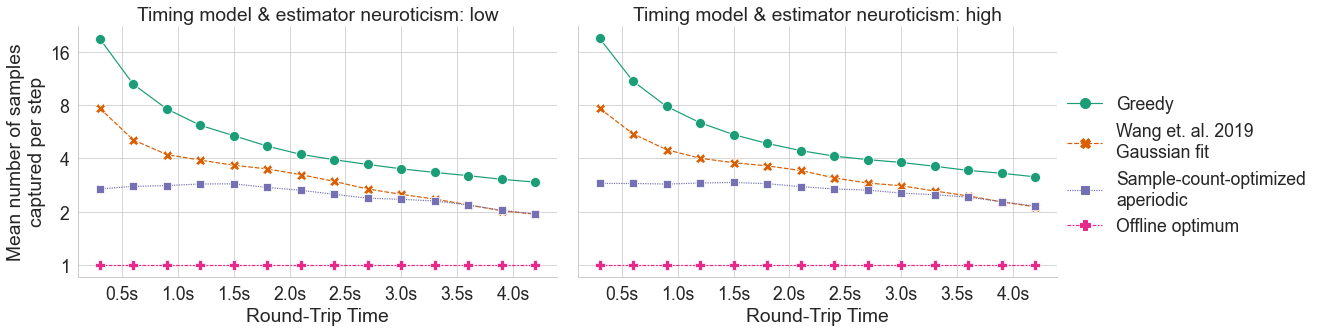
\includegraphics[width=\textwidth]{figs/new_model/sampling_optimization.png}
        \caption{%
            Round-trip time versus mean number of captured samples per step, averaged over all \num{100} repetitions of the experiment.
            Note the logarithmic scale on the vertical axis.
            Error bars indicate \SI{95}{\percent} \glspl{CI}.
        }
    \end{subfigure}\\
    \medskip
    \begin{subfigure}[t]{\textwidth}
        \centering
        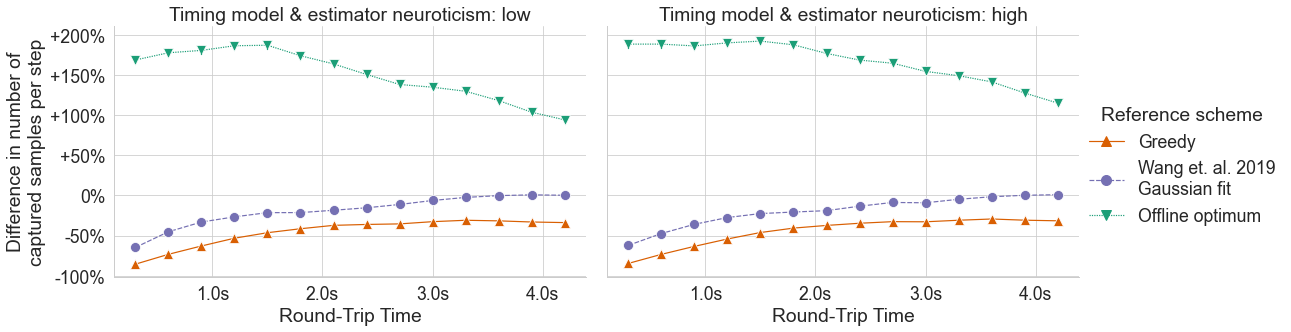
\includegraphics[width=\textwidth]{figs/new_model/sampling_optimization_diff.png}
        \caption{%
            Percentage difference in mean number of captured samples per step by the sample-count-optimized approach with respect to the three reference schemes.
            In other words, curves represent the relative performance of the sample-count-optimized scheme when using the corresponding reference scheme as baseline.
            Error bars indicate \SI{95}{\percent} \glspl{CI}, calculated using a two-sided t-test.
        }
    \end{subfigure}
    \caption{%
        Summary of results for experiment comparing the sample-count-optimized aperiodic sampling scheme to the reference schemes and \textcite{wang2019towards}'s \gls{CDF}-based approach.
    }\label{fig:optimization:samples}
\end{figure*}

The results of this investigation are presented in \cref{fig:optimization:samples}, and clearly show the advantages of using the sample-count-optimized scheme over the current state-of-the-art.
The performance of \textcite{wang2019towards}'s approach appears to degrade with lower \glspl{RTT}, exponentially oversampling as latency tends to zero and the maximum sampling rate of the system tends to infinity.
On the other hand our sampling scheme consistently matches or beats the state-of-the-art while maintaining a relatively constant behavior with respect to \glspl{RTT}.
As mentioned above, the future feasibility and mass adoption of \gls{WCA} depends on these applications not hogging the available resources.
Our work advances this goal by being consistently more efficient than existing alternatives at minimizing the number of samples per step, and thus reducing network and processing load.

It should be noted that although both schemes seem to tend towards two samples per step as \glspl{RTT} increase, this is simply an artifact of our experimental setup.
As \glspl{RTT} increase above the expected wait time, the probability of the sum of the first sampling interval and the \gls{RTT} being larger than the execution time of the step tends towards \num{1.0}.
This leads to these sampling schemes consistently sampling only twice each step: a first sample which is taken before the execution time of the step, and a second one \gls{RTT} seconds later, after the execution time has been reached.

\subsection{Optimizing for energy consumption}\label{ssec:optimization:energy}

Next we will explore the implications of combining our timing models with \cref{eq:epsilon_terminal} when directly optimizing for energy consumption in \gls{WCA}.
Although, as mentioned above, minimizing the number of samples captured during a step can \emph{potentially} translate into a reduction in the energy consumption, this is not a given.
Energy consumption depends on multiple other factors other than number of samples captured, such as idle versus communication power and delays, and thus cannot be optimized by simply minimizing the number of samples taken.

In the following, we thus take the general solution, \cref{eq:epsilon_terminal}, and find the appropriate \( \alpha \) and \( \beta \) to minimize the energy consumed per step, i.e.\ \( \mathcal{E}=E \).
We directly take the modeling from~\cite{moothedath2022energy2} with a necessary modification in the  assumption of one-way communication in all but the final sample.
With feedback given even to the discarded samples in our model and communication delay defined as the total delay in either direction, we have, 
\begin{alignat}{2}
    \mathrm{E}=&\;\mathcal{S}\tau_cP_c+(\mathcal{T}+\mathcal{W}+\tau_\mathrm{p}+\tau_\mathrm{c}-\mathcal{S}\tau_c)P_0\nonumber\\
    % &=s\tau_c(P_c-P_0^{(t)})+wP_0^{(t)}+(\tau+\tau_c+\tau_p) P_0^{(t)}+\tau_cP_c\\
    =&\;\tau_{\text{c}}(P_{\text{c}} -P_0)\mathcal{S}+\mathcal{W}P_0+(\mathcal{T}+\tau_{\text{p}} +\tau_{\text{c}}) P_0\nonumber\\
&\Rightarrow \alpha=\tau_{\text{c}}(P_{\text{c}} -P_0),\text{ and }\beta=P_0 \label{eq:optimization:energy}
\end{alignat}
\( \tau_\text{p} \) and \( \tau_\text{c} \) correspond to the processing and two-way communication delay for each sample.
\( P_\text{c} \) and \( P_0 \) correspond to the communication and idle power, respectively, of the \gls{WCA} client device.

We proceed to repeat the experiment detailed in \cref{ssec:optimization:samples}, replacing the sample-count-optimized sampling scheme with a new implementation instead minimizing energy, using \cref{eq:optimization:energy} for the calculation of \( \alpha \) and \( \beta \).
Once again, we embed a timing model into the sampling scheme to provide updated estimates of the mean execution time \( \mu \) at each step.
We refer to this scheme as the \emph{energy-optimized aperiodic} sampling scheme.
For the power constants, we reuse the values estimated by the authors in~\cite{moothedath2022energy1}, \( P_\text{c} = 45\,\si{\milli\watt} \) and \( P_\text{0} = 15\,\si{\milli\watt} \).
On the other hand, for the timing variables we define a constant processing delay \( \tau_\text{p} = 250\,\si{\milli\second} \) across all configurations and repetitions of the experiments; given then a constant \gls{RTT} for the task, we set \( \tau_\text{c} = \text{\gls{RTT}} - \tau_\text{p} \).

\begin{figure*}
    \centering
    \begin{subfigure}[t]{\textwidth}
        \centering
        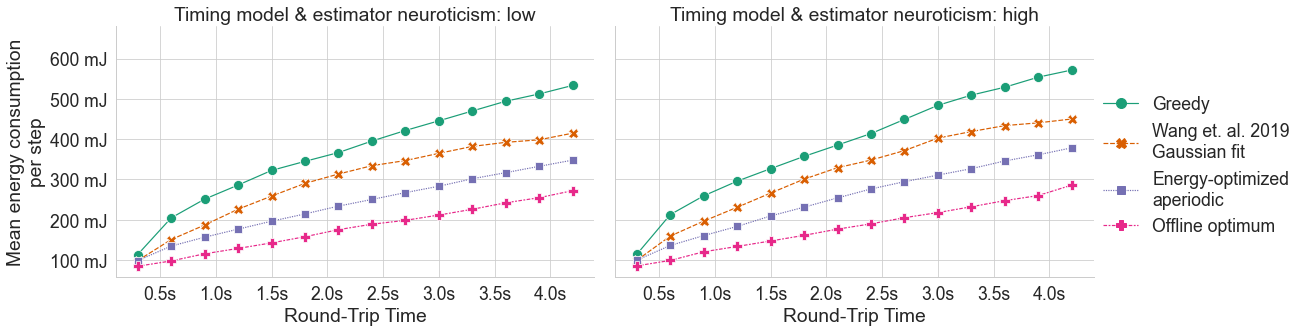
\includegraphics[width=\textwidth]{figs/new_model/energy_optimization.png}
        \caption{%
            Round-trip time versus mean per step energy consumption, averaged over all \num{100} repetitions of the experiment.
            Error bars indicate \SI{95}{\percent} \glspl{CI}.
        }
    \end{subfigure}\\
    \medskip
    \begin{subfigure}[t]{\textwidth}
        \centering
        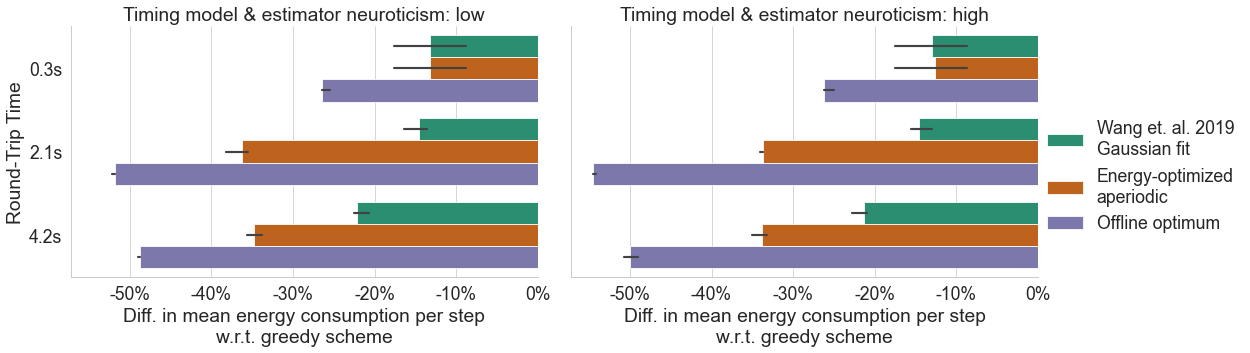
\includegraphics[width=\textwidth]{figs/new_model/energy_optimization_diff.png}
        \caption{%
            Percentage difference in mean per step energy consumption by the energy-optimized sampling scheme with respect to the three reference schemes.
            Error bars indicate \SI{95}{\percent} \glspl{CI}, calculated using a two-sided t-test.
        }
    \end{subfigure}
    \caption{%
        Summary of results for experiment comparing the energy-optimized aperiodic sampling scheme to the reference schemes and \textcite{wang2019towards}'s \gls{CDF}-based approach.
    }\label{fig:optimization:energy}
\end{figure*}

Again, we include the reference greedy and offline optimum schemes, as well as \textcite{wang2019towards}'s approach, and repeat the experiment \num{100} times for each combination of sampling scheme, neuroticism, and \gls{RTT}.

The results of these experiments are presented in \cref{fig:optimization:energy}, and they clearly illustrate the advantages of the integration of our timing models with an adaptive, energy-optimized sampling scheme when compared to unoptimized and state-of-the-art sampling schemes.
Our approach is consistently consumes \SI{20}{\percent} less energy than \textcite{wang2019towards}'s state-of-the-art, and is up to \SI{40}{\percent} more energy efficient than the greedy scheme.
Furthermore, once again the behavior of our approach is more consistent and reliable than the competition, exhibiting a flat curve of energy consumption much akin to that of the offline optimum in behavior.

\section{Discussion}\label{sec:discussion}

\subsection{Optimizing systems for \ac{WCA}}

\section{Conclusion}\label{sec:conclusion}

The study and benchmarking of \ac{WCA} applications is a challenging discipline due to these application's intrinsic human-in-the-loop nature.
Humans are notoriously unreliable, and greatly complicate the scalability and repeatability of experiments.
Furthermore, recruiting large enough cohorts of humans for large-scale experimentation is both greatly time-consuming and prohibitively expensive for many research groups.

In the first half of this paper, we have introduced the \edgedroid{} model of human timing behavior for \ac{WCA}, the first data-driven model for human timings in \ac{WCA} applications.
This model represents a stochastic approach to execution time modeling which builds upon the data collected for \textcite{olguinmunoz:impact2021}.
Together with this model, we have also introduced a novel procedure for the generation of synthetic traces of frames in step-based \ac{WCA}, allowing for a full end-to-end emulation of a human when combined with the timing model.

In the second half, we have explored the potential for optimization in \ac{WCA} systems using the previously discussed timing models.
We have proposed a novel stochastic optimization framework for resource consumption-system responsiveness trade-offs in \ac{WCA}.
We have shown that this framework is applicable to a myriad of parameters in these applications, and showcased experimental results employing this framework for the minimization of number of samples processed per step and total energy consumption per step.
Our results show up to a \SI{50}{\percent} increase in performance with respect to state of the art when optimizing for number of samples, and up to a \SI{30}{\percent} improvement when optimizing for energy consumption, proving thus the value of such frameworks for the design of \ac{WCA} applications.

\todo[inline]{Finish}
\section*{Acknowledgements}\label{sec:acks}

This work has been partially funded by the \gls{SSF} (grant number \verb|ITM17-0246| (ExPECA)), and the \gls{NSF} (grant number \verb|CNS-2106862|).
The funders had no role in study design, data collection and analysis, decision to publish, or preparation of the manuscript.
Any opinions, findings, conclusions or recommendations expressed in this material are those of the authors and do not necessarily reflect the view(s) of their employers or funding sources.
% \section{Aperiodic Sampling}

In this section we will explain the method that we used to find the optimum set of sampling instants (or equivalently sampling intervals) for the given distribution of TTE, denoted by $\mathcal{T}$.
\todo[inline]{aka execution times. Need to recheck the terminologies used in this section and make it consistent with the paper.}
We take the modeling and partial solution approach from the recent works on energy efficient sampling of edge-based feedback systems.
In \textcite{ICCperiodic1,TMCperiodic}, the authors model the energy in terms of the expected number of samples $\mathbb{E}[\mathcal{S}]$ and the expected wait time $\mathbb{E}[\mathcal{W}]$ experienced by the user, where the wait time $\mathcal{W}$ --- in the terminology of the authors --- is the time between the event completion and the immediate next sample taken.
The authors then find the optimum periodic sampling interval that minimizes this energy, or equivalently the non-constant parts of this energy termed as \textit{Energy Penalty} $\mathcal{E}$.
In this optimization, the constant parts are excluded as they do not affect the optimization.
With a value much smaller than the execution time of the event or TTE, the RTT of the final sample is included in this constant part, which is the reason why $\mathcal{W}$ is computed without including this RTT.
Next, in \textcite{secAperiodic}, the authors use this exact model and find the optimum aperiodic sampling instants $\{t_n,\,n=1,2,\dots\}$ that minimizes the same energy penalty.
In this work, we use the modeling from \textcite{secAperiodic} to find the optimum aperiodic sampling interval.
However, instead of using their two-step approach to find the solution which include a recursive solution followed by an algorithm, we develop a novel approximate but easier solution to finding the set of optimum aperiodic sampling intervals.
In what follows, we first recap the system modeling used by the authors in \textcite{secAperiodic} and then give our independent approximate solution. 

The energy penalty can be expressed as~\cite{secAperiodic}
\begin{alignat}{1}
\Rightarrow\mathcal{E}&=\alpha\mathbb{E}[\mathcal{S}]+\beta\mathbb{E}[\mathcal{W}],\;\label{eq:epsilon_terminal}
\end{alignat}
where $\alpha\!=\!\tau_{\text{c}} (P_{\text{c}}\!-\!P_0)$ and $\beta\!=\!P_0$ are constants.
\todo[inline]{Define and explain the parameters if this is not done earlier in other sections.}
Here, note that $\alpha\mathbb{E}[\mathcal{S}]$ and $\beta\,\mathbb{E}[\mathcal{W}]$ corresponds to the energy wasted per discarded sample and the additional energy expended for waiting, respectively.
As noted down by the authors, it is important to note that this optimization approach can also be applied to optimize metrics other than energy, simply by formulating this new metrics in the same format as follows, that is by expressing the metric as a linear combination of the expected number of samples $\mathbb{E}[\mathcal{S}]$ and expected wait time $\mathbb{E}[\mathcal{W}]$.
Using this model, we find the approximate, near-optimal set of sampling instants $\{t_n^*\}$ that minimizes the energy penalty given in \cref{eq:epsilon_terminal}.


\subsection{Optimum sampling instants}\label{sec:aprxSol}

First, we borrow the idea of checkpointing density from \textcite{CP_C} and call it instantaneous sampling rate function $r(t)$ which is
related to $\{t_n\}$ such that,
\begin{alignat}{1}
{\int_{t_{n-1}}^{t_n}}r(t)\dif t=1,\;\forall n\geq1.\label{rt}
\end{alignat}
We find $r^*(t)$, the $r(t)$ that minimizes $\mathcal{E}$.
Note that, by construction, the number of samples taken up to any time instant can be computed directly by finding the area under $r(t)$.
Thus, we get the expected number of samples $\mathbb{E}[\mathcal{S}]$ as
\begin{alignat}{1}
\mathbb{E}[\mathcal{S}]&=\int_{t=0}^{\infty}\bigg(\!\int_{x=0}^{t}\!\!\!\!r(x)\,\mathrm{d}x\bigg)f_{\mathcal{T}}(t)\,\mathrm{d}t.\label{Es}
\end{alignat}
To find 
% the expected wait 
$\mathbb{E}[\mathcal{W}]$, we use the TTE conditional CDF.
We get,
\begin{multline*}
\mathbb{P}(\mathcal{W}=t_n-\mathcal{T}\leq t\,\big\vert\,t_{n-1}<\mathcal{T}\leq t_n)\\=\dfrac{\mathbb{P}(\mathcal{T}\geq t_n-t\,,\,t_{n-1}<\mathcal{T}\leq t_n)}{\mathbb{P}(t_{n-1}<\mathcal{T}\leq t_n)}.
\end{multline*}
The numerator is degenerate when $t\!<\!0$ or $t\!>\!(t_n\!-\!t_{n-1})$.
Thus, we are only interested in $0\!\leq\!t\!\leq\! (t_n-t_{n-1})$.
Let $F_{\mathcal{T}}$, $\bar{F}_{\mathcal{T}}$ and $f_{\mathcal{T}}$ corresponds to the CDF, CCDF and pdf of the TTE distribution.
\begin{alignat*}{1}
\!\!\!\Rightarrow\mathbb{P}(\mathcal{W}\leq t\,\big\vert\,t_{n-1}<\mathcal{T}\leq t_n)&=\dfrac{\mathbb{P}(t_n-t\leq\mathcal{T}\leq t_n)}{F_\mathcal{T}(t_n)-F_\mathcal{T}(t_{n-1})}\\
&\approx\dfrac{F_\mathcal{T}(t_n)-F_\mathcal{T}(t_{n}-t)}{F_\mathcal{T}(t_n)-F_\mathcal{T}(t_{n-1})}\tag{$A_1$}\label{Apx1}
\end{alignat*}
Here, \ref{Apx1} is an approximation merely for mathematical maturity due to the slackness of the first inequality in the numerator.
Expanding the CDF using Taylor series, 
\begin{multline*}
    =\Big(F_\mathcal{T}(t_n)-\big(F_\mathcal{T}(t_n)+f_\mathcal{T}(t_n)(-t)+f'_\mathcal{T}(t_n)(-t)^2/2!+\dots\big)\Big)\\
    \div \Big(F_\mathcal{T}(t_n)-\big(F_\mathcal{T}(t_n)+f_\mathcal{T}(t_n)(t_{n-1}-t_n)\\+f'_\mathcal{T}(t_n)(t_{n-1}-t_n)^2/2!+\dots\big)\Big).
\end{multline*}
Simplifying and using the first order approximation, we get
\begin{alignat*}{1}
% &=\dfrac{F_\mathcal{T}(t_n)-\big(F_\mathcal{T}(t_n)+f_\mathcal{T}(t_n)(-t)+f'_\mathcal{T}(t_n)(-t)^2/2!+\dots\big)}{F_\mathcal{T}(t_n)-\big(F_\mathcal{T}(t_n)+f_\mathcal{T}(t_n)(t_{n-1}-t_n)+f'_\mathcal{T}(t_n)(t_{n-1}-t_n)^2/2!+\dots\big)}\\&
\mathbb{P}(\mathcal{W}\leq t\,\big\vert\,t_{n-1}<\mathcal{T}\leq t_n)&\approx\dfrac{tf_\mathcal{T}(t_n)}{(t_{n}-t_{n-1})f_\mathcal{T}(t_n)}\tag{$A_2$}\label{Apx2}\\
\Rightarrow\mathbb{P}(\mathcal{W}> t\,|\,t_{n-1}<\mathcal{T}\leq t_n)&= 1-\dfrac{t}{(t_{n}-t_{n-1})}.
\end{alignat*}
Using this CCDF, we find the conditional expectation of $\mathcal{W}$.
\begin{alignat*}{1}
% \mathbb{P}(\mathcal{W}> t\,|\,t_{n-1}<\mathcal{T}\leq t_n)&\approx 1-\dfrac{t}{(t_{n}-t_{n-1})}\\
\Rightarrow \mathbb{E}[\mathcal{W}\,|\,t_{n-1}<\mathcal{T}\leq t_n]&=\smashoperator[r]{\int_{0}^{t_n-t_{n-1}}}\Big(1-\dfrac{t}{(t_{n}-t_{n-1})}\Big)\,\mathrm{d}t\\
&=\dfrac{(t_n-t_{n-1})}{2}.
\end{alignat*}
% However, we can also approximate $(t_n-t_{n-1})$, the sampling interval to the inverse of the instantaneous sampling frequency $r(t)$. This approximation (\ref{Apx3}) is valid as long as $r(t)$ is varying slowly between two consecutive sampling instants. That is,
If $r(t)$ is varying slowly between two consecutive sampling instants, we can approximate the sampling interval $t_n\!-\!t_{n-1}$ as,
\begin{alignat}{1}
 (t_n-t_{n-1})&\approx\dfrac{1}{r(t)},\;\forall t,n:t_{n-1}\!<\!t\!\leq\!t_n.\tag{$A_3$}\label{Apx3}\\
% \end{alignat}
% As a result, we can compute the expected wait as,
% \begin{alignat}{1}
\Rightarrow \mathbb{E}[\mathcal{W}]&=\int_{0}^{\infty}\mathbb{E}[\mathcal{W}\,|\,t_{n-1}<\mathcal{T}\leq t_n]f_\mathcal{T}(t)\,\mathrm{d}t\nonumber\\
&=\int_{0}^{\infty}\dfrac{1}{2r(t)}f_\mathcal{T}(t)\,\mathrm{d}t.\label{Ew}
\end{alignat}
We can thus find the energy penalty using \eqref{Es} and \eqref{Ew} as
\begin{alignat*}{1}
\mathcal{E}&=\int_{0}^{\infty}\Big(\alpha\int_{x=0}^{t}r(x)\,\mathrm{d}x+\beta\dfrac{1}{2r(t)}\Big)f_{\mathcal{T}}(t)\,\mathrm{d}t.\label{epsilon_eulerForm}\\
\intertext{Let $g(t)=\int_{0}^{t}r(x)\dif x$. Then  $g'(t)=\tfrac{\mathrm{d}}{\mathrm{d}t}g(t)=r(t)$. That is,}
\vspace{-4cm}\mathcal{E}&=\int_{0}^{\infty}\Big(\alpha g(t)+\dfrac{\beta}{2g'(t)}\Big)f_{\mathcal{T}}(t)\,\mathrm{d}t.
\end{alignat*}
As per the Euler-Lagrange equation from the calculus of variations\cite{calcVariation2,calcVariation1}, the extreme value of $\mathcal{E}$ is obtained at 
\begin{alignat}{1}
r^*(t)&=\sqrt{\dfrac{\beta f_\mathcal{T}(t)}{2\alpha\bar{F}_\mathcal{T}(t)}}.\\
\intertext{Thus, for a Rayleigh distributed $\mathcal{T}$ with parameter $\sigma$,}
r^*(t)&=\sqrt{\dfrac{\beta t}{2\alpha\sigma^2}}\\
\Rightarrow &\int_{t_n}^{t_{n+1}}\!\!\!\sqrt{\dfrac{\beta t}{2\alpha\sigma^2}}\,\mathrm{d}t=1,\;\forall n\geq1\nonumber\tag{from \eqref{rt}}\\
\Rightarrow &\;t_{n+1}^{\frac{3}{2}}-t_{n}^{\frac{3}{2}}=3\sigma\!\sqrt{\tfrac{\alpha}{2\beta}}\nonumber\\
\Rightarrow &\;t_n=\Big(3\sigma\!\sqrt{\tfrac{\alpha}{2\beta}}\Big)^{\frac{2}{3}}n^{\frac{2}{3}}.\label{tnFinal}
\end{alignat}

Now, if we have a constrained optimization with an upper bound $w_0$ for the expected wait time, we can find the optimum set of sampling instants by equating \cref{Ew} to $w_0$ and find the ratio of $\frac{\alpha}{\beta}$ that provides the optimum set of sampling instants when plugged into \cref{tnFinal}.
For this, we make use of the facts that
\begin{enumerate*}[itemjoin={{, }}, itemjoin*={{, and }}]
    \item the bound will be tight at the optimum due to the continuous nature of possible sampling instants and sampling intervals
    \item one can achieve any arbitrary point $(\mathbb{E}[\mathcal{S}],\mathbb{E}[\mathcal{W}])$ via the unconstrained optimization discussed above simply by varying the ratio $\frac{\alpha}{\beta}$.
\end{enumerate*}
\begin{alignat*}{1}
\mathbb{E}[\mathcal{W}]&=\int_{0}^{\infty}\dfrac{1}{2r(t)}f_\mathcal{T}(t)\,\mathrm{d}t.\nonumber\\
&=\int_{0}^{\infty}\frac{1}{2}\sqrt{\frac{2\alpha\sigma^2}{\beta t}}\cdot \frac{t}{\sigma^2}e^{-{t^2}/{2\sigma^2}}\mathrm{d}t\\
&=\sqrt{\frac{\alpha\sigma^2}{2\beta}}\int_{0}^{\infty}\frac{\sqrt{t}}{\sigma^2}e^{-{t^2}/{2\sigma^2}}\mathrm{d}t\\
&=\sqrt{\frac{\alpha\sigma^2}{2\beta}}\left({\frac{1}{{2}\sigma^2}}\right)^{1/4}\cdot\int_{0}^{\infty}y^{-1/4}e^{-y}\mathrm{d}y\\
&=\sqrt{\frac{\alpha\sigma^2}{2\beta}}\left({\frac{1}{{2}\sigma^2}}\right)^{1/4}\cdot\mathlarger{\Gamma}(\tfrac{3}{4})\\
% &\approx 0.728637\sqrt{\frac{\alpha\sigma}{\beta}}\\
\intertext{Thus, when the upper bound $w_0$ is tight,}
w_0&=0.728637\sqrt{\frac{\alpha\sigma}{\beta}}\\
w_0&=\sqrt{\frac{\alpha\sigma}{2\sqrt{2}\beta}}\mathlarger{\Gamma}(\tfrac{3}{4})\\
\Rightarrow\frac{\alpha}{\beta}&=\frac{w_0^2}{\sigma}\frac{2\sqrt{2}}{(\mathlarger{\Gamma}(\tfrac{3}{4}))^2}\\&=1.88355\frac{w_0^2}{\sigma}
\end{alignat*}

Now, we modify the problem and find the optimum sampling instants that minimises the number of samples for a given upper bound for the e
\printbibliography{}
\newpage%
\appendices
\section{Moderation of effects by individual characteristics}\label{ssec:moderationeffects}

In~\cite{olguinmunoz2021impact}, we recorded variables related to well-known individual differences, encompassing both the \glspl{BFI}~\cite{john1999big}, and the \glspl{ITQ}~\cite{witmer1998measuring}.
Out of the individual-difference variables, the most salient effect on performance corresponded to \emph{neuroticism}, a \gls{BFI} trait linked to low tolerance for stress and high emotional reactivity, and which has previously been linked to higher \emph{delay discounting} rates~\cite{hirsh2008delay}.
Delay discounting is the tendency to devalue rewards for which one must wait; high rates, indicative of waiting intolerance, have been associated with negative social and academic outcomes.

% Bobby suggested we remove this figure and just give the pearson coeff.
% \begin{figure}
%     \centering
%     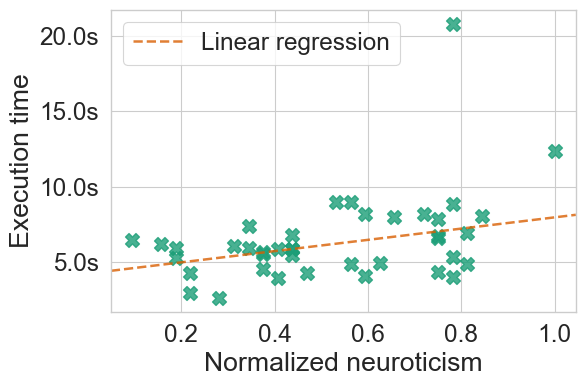
\includegraphics[width=\textwidth]{figs/new_model/correlation_neuro_exectime.png}
%     \caption{%
%         Correlation between neuroticism and the mean execution time of the last four steps in segments of \num{12} steps subject to the same \gls{TTF} in~\textcite{olguinmunoz:impact2021}.
%         Pearson correlation coefficient \( \rho = 0.418 \), 2-tailed \( p < 0.05 \).
%     }\label{fig:neuroexectimecorrel}
% \end{figure}

% In this work, we have used a normalized scale to describe neuroticism, derived from the minimum and maximum obtainable values for this variable in the \gls{BFI}~\cite{john1999big}.
% \emph{Low} and \emph{high} neuroticism refer to the \( [0.0, 0.5) \) and \( [0.5, 1.0] \) ranges respectively.

Linear regression showed a significant correlation between individual neuroticism scores and the execution time late in a series of high-delay steps, \( \rho = 0.418 \), \num{2}-tailed \( p < 0.05 \)
Neuroticism was further identified as a modulating factor for the pacing effects through a \gls{PCA}.
Out of the three identified components, which cumulatively accounted for \SI{73.13}{\percent} of the variance in the results, neuroticism was included in the first two.
The effect of neuroticism was observed across all \glspl{TTF} and impairment durations in the tasks.

Furthermore, we found that execution times, when grouped by experimental variables such as neuroticism, \gls{TTF}, and continuous segments of steps subject to the same \gls{TTF}, were well-fit by an \gls{exGaussian} distribution, as verified using Kolmogorov-Smirnov goodness-of-fit tests~\cite{massey_jr1951kolmogorov}.
When grouping by level of neuroticism, \gls{TTF}, and \emph{slice}\footnote{%
In~\cite{olguinmunoz2021impact} the \emph{slice} to which a step belongs to refers to whether the step occurred in the first, second, or third four-step segment of a sequence of steps subject to the same \gls{TTF}.
}, the best fit statistic was \ensuremath{0.028} (\ensuremath{p = 0.999}).
This distribution has an ample body of research supporting its suitability for the modeling of the timing of human actions and reaction times~\cite{rohrer1994analysis,palmer2011what,marmolejo_ramos2022generalised}.
We found that the effects of neuroticism on execution times were clearly identifiable in the fitted distributions, in particular in their means and tails.
\cref{fig:muexgaussian} shows an example of this modulating effect, illustrating the behavior of the mean (\( \mu \) parameter) of \gls{exGaussian} distributions fitted to the execution times of the first four steps of segments of steps subject to the same \gls{TTF}.
Finally, \cref{fig:fitsneuro} shows an example of the effects of neuroticism on the fitted \gls{exGaussian} distributions for a specific group of execution times.
Higher neuroticism directly translates into a higher mean and longer tail.

\begin{figure}
    \centering
    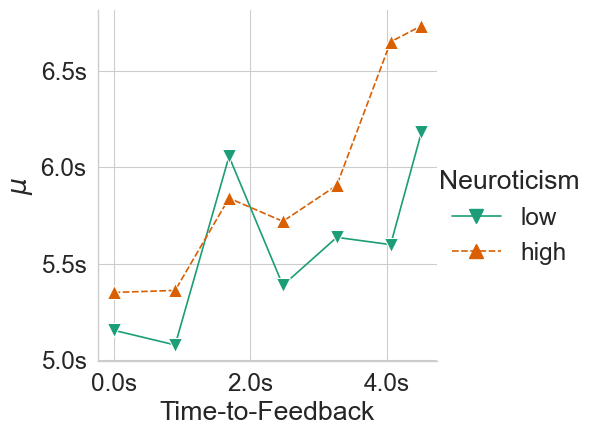
\includegraphics[width=.9\columnwidth]{figs/new_model/mu_fits_exgaussian_slice0}
    \caption{%
        \( \mu \) parameter of \gls{exGaussian} distributions fitted to execution times of the first four steps of segments of steps subject to the same \gls{TTF} in~\cite{olguinmunoz2021impact}.
        Distributions were fitted using \gls{MLE}.
    }\label{fig:muexgaussian}
\end{figure}

\begin{figure}
    \centering
    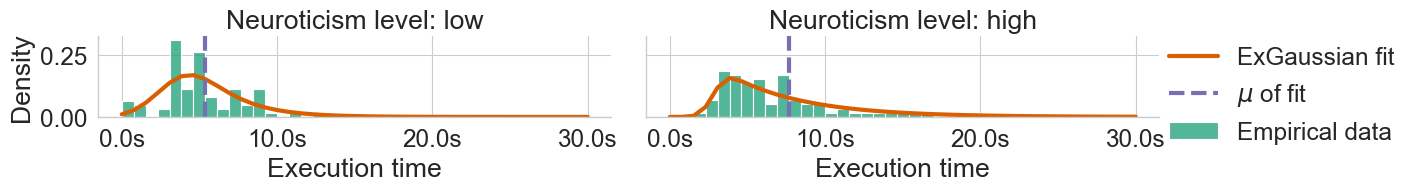
\includegraphics[width=.9\columnwidth]{figs/new_model/dist_fits_neuro}
    \caption{%
        Example \gls{exGaussian} fits on execution times from steps \numrange{4}{8} in a segment of steps at the maximum experimental \gls{TTF}.
        The effects of neuroticism are clearly visible in the tail and the mean of the distributions.
    }\label{fig:fitsneuro}
\end{figure}

\end{document}
